\documentclass[conference]{IEEEtran}
\IEEEoverridecommandlockouts

\usepackage{cite}
\usepackage{amsmath,amssymb,amsfonts}
\usepackage{algorithmic}
\usepackage{graphicx}
\usepackage{textcomp}
\usepackage{xcolor}
\usepackage{booktabs}
\usepackage{tabularx}
\usepackage{array}
\usepackage{url}
\usepackage{microtype}

\begin{document}

\title{Freshness-Aware, Provenance-Tracked Healthcare Resource Discovery in Fragmented Urban Ecosystems: System Design, Staleness Dynamics, and Transactional Evaluation}

\author{
\IEEEauthorblockN{MedReach Research Collaboration}
\IEEEauthorblockA{\textit{Department of Health Informatics and Systems Engineering} \\
\textit{Urban Healthcare Systems Initiative}\\
Mumbai, Maharashtra, India \\
contact@medreach.local}
}

\maketitle

\begin{abstract}
Locating emergency healthcare resources---such as intensive care unit (ICU) beds, specialized surgical facilities, and compatible blood components---in dense, fragmented metropolitan centers like Mumbai represents a critical coordination challenge. Traditional civilian search relies on phone inquiries, unverified static directories, or physical transit between casualty wards, consuming the clinical ``golden hour'' and exacerbating emergency department crowding. While digital health platforms have emerged, existing regional platforms operate almost exclusively as unverified static directories or asynchronous self-reported bulletins, lacking freshness tracking, provenance fusion, and two-way confirmation.

This paper presents an architectural design and comprehensive empirical evaluation of MedReach, an open-source, freshness-aware, and provenance-tracked emergency resource discovery platform designed for urban healthcare coordination. MedReach establishes a decoupled, multi-tiered data model that enforces explicit Age of Information (AoI) boundaries, multi-source provenance fusion with priority cascades, and idempotent state-machine workflows for two-way clinical requests. 

Through extensive empirical evaluation across five experimental suites, we report:
(1) In a synthetic simulation suite across 6 operational archetypes (300 trajectories, 1,296,000 query evaluations over 72-hour operational horizons), MedReach's pre-registered 30-minute availability cutoff ($\tau = 30\text{ min}$) functions as a critical clinical safety governor. Under manual 2-hour shift reporting, the 30-minute threshold withholds status 78.42\% of the time, keeping dangerous ``phantom availability'' (displaying beds as available when physically full) down to 0.337\%. Loosening the cutoff to 180 minutes expands coverage to 97.15\% but causes phantom availability to explode by 18.9$\times$ to 6.382\% with an overall status error rate of 53.71\%. When updates are collected via batch crawlers with 15--45 min queue latency, 51.79\% of updates arrive already stale at 30 minutes, and 99.64\% arrive stale at 10 minutes.
(2) Evaluating the production fusion engine against 40,000+ synthetic trials with known ground truth reveals a 100.0\% conflict detection rate and 90.29\% conditional resolution accuracy. However, calibration analysis reveals an essential negative finding: MedReach's confidence metric is an uncalibrated heuristic ordinal ranking (Brier score 0.1315, Expected Calibration Error 0.1255, Maximum Calibration Error 0.7333) rather than a calibrated Bayesian probability.
(3) An architectural audit of 22 deployed endpoints resolves an earlier theoretical concern: edge-cached prerendered HTML shells served with multi-hour retention contain zero volatile capacity data (structural DOM shells only), with all live availability fetched dynamically at runtime via client-side React hooks, entirely refuting the static-page staling hazard (verdict: NOT SUPPORTED).
(4) In an isolated suite of 48 test assertions evaluating concurrency and idempotency, the platform achieved a 100.0\% pass rate, demonstrating strict request deduplication via SHA-256 scoped idempotency keys and optimistic concurrency control under 10-way concurrency.
(5) Single-machine loopback load benchmarking via \texttt{autocannon} 8.0.0 demonstrates that baseline database reads (\texttt{GET /api/hospitals}) sustain 284.7 req/s (median latency 3.00 ms, $p_{99} = 9.67\text{ ms}$), saturating at ~395 req/s at concurrency $C=50$, cleanly absorbing an instantaneous 50$\times$ surge ($C=250$, 386.7 req/s) with zero connection drops, and recovering to 2.0 ms median latency.

We provide a comprehensive two-column architectural analysis detailing demonstrable system guarantees versus components still requiring implementation, establishing an evidence-based foundation for resilient urban health infrastructure.
\end{abstract}

\begin{IEEEkeywords}
Age of Information (AoI), Data Freshness, Emergency Healthcare Informatics, Idempotency, Multi-Source Data Fusion, Provenance Tracking, Resource Discovery, Transactional Reliability.
\end{IEEEkeywords}

\section{Introduction}

In dense urban agglomerations in low- and middle-income countries (LMICs), acute emergency healthcare access remains severely constrained by information friction \cite{metuge2026digital,dalton2019patient}. When a patient suffers severe polytrauma, acute respiratory failure, or obstetric hemorrhage in Mumbai---a metropolitan area exceeding 13 million residents---locating an operational intensive care unit (ICU) bed, a mechanical ventilator, or an appropriate blood component unit is a high-stakes coordination problem \cite{darapaneni2021predicting,naydenova2017healthcare}. 

The urban healthcare landscape in Mumbai is exceptionally pluralistic and fragmented: it comprises municipal medical colleges (e.g., KEM, Sion, Nair, Cooper) managed by the Municipal Corporation of Greater Mumbai (MCGM), state government hospitals (e.g., Sir J.J. Group), charitable trust institutions (e.g., Lilavati, Bombay Hospital, Hinduja), and hundreds of private corporate centers and nursing homes \cite{shinde2026insights,mcgm2021covidwarroom,more2009inequalities}. In the absence of a unified, real-time dispatch and bed-tracking system, citizens, private ambulance operators, and primary clinic physicians traditionally engage in exploratory manual searching---placing repeated telephone calls to casualty departments or physically transporting patients between emergency rooms \cite{patil2016study,mukhopadhyay2018stroke}. This exploratory process frequently consumes the clinical ``golden hour'', induces catastrophic secondary inter-facility transfers, and increases risks for time-critical conditions \cite{naydenova2017healthcare,darapaneni2021predicting,skordisworrall2011maternal}.

Although public web portals exist---including the Brihanmumbai Municipal Corporation (BMC) health dashboard and the national e-RaktKosh blood transfusion registry---empirical investigation demonstrates that they operate primarily as static directory listings or asynchronous, unverified inventory bulletins \cite{metuge2026digital,mohfw2022eraktkosh}. They lack automated freshness tracking, provide zero information regarding verification provenance, and offer no mechanism for two-way clinical confirmation or reservation holds \cite{haeder2023state,haeder2024consumer}. Consequently, healthcare searchers frequently encounter ``phantom availability'': digital platforms advertise available beds or blood units that were exhausted hours earlier, leading to tragic misdirection.

To address this challenge, the \textbf{MedReach} platform was developed as an open-source, freshness-aware, and provenance-tracked discovery and two-way coordination system. MedReach introduces three core architectural mechanisms:
\begin{enumerate}
    \item \textbf{Freshness-Aware Availability Tracking}: A deterministic evaluation engine that tracks the exact Age of Information (AoI) of resource telemetry and automatically demotes stale observations to \texttt{"unknown"} beyond a strict 30-minute threshold (\texttt{CURRENT\_AVAILABILITY\_MAX\_AGE\_MS = 30 * 60 * 1000}), refusing to present unverified point-in-time capacity as guaranteed care \cite{kaul2012realtime,yates2021age}.
    \item \textbf{Provenance-Aware Conflicting-Claim Fusion}: A deterministic priority cascade that tracks source reliability, verification status, and timestamps, detecting divergent claims across official APIs, hospital web scrapers, and manual audits, and deferring unresolved institutional disputes to safe ignorance rather than algorithmic guesswork \cite{bleiholder2008data,dong2009data,moreau2011open}.
    \item \textbf{Idempotent, Two-Way Request Orchestration}: A state-machine transaction model that decouples observational capacity telemetry from request fulfillment, protecting emergency requests against network retries, duplicate submissions, and race conditions via SHA-256 scoped idempotency keys and optimistic concurrency control (OCC).
\end{enumerate}

\section{Background and Related Work}

\subsection{Emergency Healthcare Navigation in Urban LMICs}
Emergency medical care in urban LMIC contexts faces severe operational barriers characterized by three delays: delay in seeking care, delay in reaching care, and delay in receiving definitive care \cite{dalton2019patient,skordisworrall2011maternal}. In major Indian metropolitan centers like Mumbai, emergency transport operates in a deeply divided market: public 108 ambulances, municipal hospital vehicles, and numerous uncoordinated private ambulance fleets operate without centralized telematics \cite{naydenova2017healthcare,shinde2026insights}. Consequently, patients and their relatives undertake uncoordinated searches across facilities, driving acute emergency department overcrowding in public tertiary centers while nearby peripheral facilities remain underutilized \cite{darapaneni2021predicting,patil2016study}. Digital health interventions have frequently failed to improve outcomes because they digitized directory listings without solving the underlying operational uncertainty of whether a clinical resource is actually vacant at the moment of patient arrival \cite{metuge2026digital,haeder2024persistence}.

\subsection{Age of Information (AoI) and Data Staleness}
The concept of Age of Information (AoI), originally formalized by Kaul, Yates, and Gruteser \cite{kaul2012realtime,yates2021age}, quantifies data freshness from the receiver's perspective. In status-updating systems, if a packet generated at time $U(t)$ arrives at time $t$, the AoI $\Delta(t) = t - U(t)$ grows linearly in the absence of new updates and resets upon receiving fresh data \cite{sun2017update}. In healthcare resource discovery, data staleness is not merely a quality-of-service degradation; it is a clinical safety hazard. As Zou and Ozel \cite{zou2019relative} and Hu and Chen \cite{hu2020optimal} observed, when capacity fluctuates rapidly under emergency admissions, high update throughput does not guarantee freshness if queueing or ingestion delays induce update aging. In HTTP caching, RFC 9111 \cite{fielding2022caching,fielding2022semantics} and RFC 5861 \cite{nottingham2010stale} formalize freshness lifetimes and stale-while-revalidate semantics; however, general web caching specifications do not account for the asymmetric risk where a stale ``available'' indicator can cause fatal diversion.

\subsection{Provenance, Information Fusion, and Conflict Resolution}
Data fusion from heterogeneous sources has been extensively studied in database literature \cite{bleiholder2008data,dong2009data}. When aggregating information across disparate feeds, conflicts inevitably arise due to timing differences, schema variations, or erroneous reporting \cite{moreau2011open}. In public health and provider directories, empirical studies by Haeder et al. \cite{haeder2023state,haeder2024consumer,haeder2024persistence,haeder2025network} and Burman et al. \cite{burman2022provider,elton2024provider,anon2023provider} have demonstrated widespread inaccuracy in provider directory listings, where ghost networks and inaccurate contact information impede patient care. In blood banking, Kumari and Raina \cite{kumari2019reasons} and Basavarajegowda et al. \cite{basavarajegowda2026blood} showed that fragmented stock reporting exacerbates acute blood shortages. To resolve conflicting claims without human intervention, fusion engines must track cryptographic provenance, source authority tiers, and verification timestamps \cite{vermeulen2023trust,abedin2021data,liu2024data}.

\subsection{The Mumbai Healthcare Digital Landscape: Empirical Taxonomy}
To rigorously contextualize existing regional platforms, we formulate a five-tier operational taxonomy of resource visibility:
\begin{itemize}
    \item \textbf{Tier 1 (Directory Listing)}: Static facility registry (name, address, telephone, GPS coordinates).
    \item \textbf{Tier 2 (Service Offered)}: Static catalog of clinical specialties and infrastructure (e.g., ``ICU'', ``Blood Bank'', ``CT'').
    \item \textbf{Tier 3 (Resource Reported Available)}: Asynchronous, self-reported count of vacant units (e.g., ``12 beds vacant'', ``5 units A+''). Lacks transactional guarantee, reservation hold, or freshness verification.
    \item \textbf{Tier 4 (Resource Confirmed Currently Available)}: Synchronous, verified reservation or holding lock confirmed by clinical or dispatch personnel within an active freshness window.
    \item \textbf{Tier 5 (Completed Request)}: End-to-end lifecycle orchestration: triage match, dispatch, bed hold, transit, and intake handover.
\end{itemize}

Table~\ref{tab:taxonomy} classifies existing regional platforms in Mumbai and India against this hierarchy based on empirical inspection of their live web portals and documentation \cite{mohfw2019ndhb,nha2023hfr,kadambi2026ayushman}.

\begin{table*}[t]
\centering
\caption{Five-Tier Operational Taxonomy of Healthcare Resource Visibility in Mumbai and India}
\label{tab:taxonomy}
\begin{tabularx}{\textwidth}{l p{2.2cm} X p{3.2cm} p{3.6cm}}
\toprule
\textbf{Platform / System} & \textbf{Visibility Tier} & \textbf{Operational Ingestion Mechanism} & \textbf{Freshness Tracking} & \textbf{Request Confirmation} \\
\midrule
BMC Health Dashboard (COVID Era) & Tier 1--3 & 2-hour manual ward reporting & Timestamp display only & Central War Room dispatch only \\
e-RaktKosh (National Blood Portal) & Tier 1--3 & Daily self-reported inventory & Date stamp display & Unconfirmed directory (call required) \\
MahaSBTC Blood Registry & Tier 1--3 & Periodic manual web form & Date stamp display & Unconfirmed directory listing \\
NHM HMIS / National Health Portal & Tier 1--2 & Monthly aggregated administrative audit & None (Historical record) & None \\
108 Maharashtra EMS (BVG) & Tier 1--2 & Central telephone dispatch queue & Real-time vehicle telematics & Central voice triage dispatch \\
\textbf{MedReach (This Work)} & \textbf{Tier 1--4} & \textbf{AoI decay engine + OCC state machine} & \textbf{Strict 30m AoI governor} & \textbf{Two-way idempotent request workflow} \\
\bottomrule
\end{tabularx}
\end{table*}

As demonstrated in Table~\ref{tab:taxonomy}, existing regional platforms operate strictly at Tiers 1--3. Zero existing platforms provide automated freshness governors, programmatic provenance fusion, or two-way idempotent clinical request coordination.

\section{Research Gap and Contributions}

\subsection{Research Gap}
The critical research gap in urban digital health informatics is the gulf between passive, unverified directory registries (Tiers 1--3) and verifiable, freshness-governed request coordination (Tiers 4--5). While theoretical computer science has formalized AoI decay in packet networks, and database literature has developed multi-source conflict resolution, these principles have not been unified into an open-source, deployable emergency health informatics platform capable of preventing phantom availability errors while maintaining high-throughput transactional reliability under fragmented LMIC infrastructure constraints.

\subsection{Summary of Contributions}
This paper provides an end-to-end systems and empirical evaluation of MedReach, making the following contributions:
\begin{enumerate}
    \item \textbf{Formal AoI Characterization \& Safety Governor}: We formulate the information-ageing process in emergency discovery and evaluate it across 6 realistic operational archetypes (300 trajectories, 1,296,000 queries). We prove that MedReach's 30-minute anchor prevents an 18.9$\times$ surge in phantom availability errors and characterize the ``ingestion delay trap''.
    \item \textbf{Empirical Evaluation of Multi-Source Provenance Fusion}: We execute the production claim fusion engine against 40,000+ synthetic trials with known ground truth, establishing a 100.0\% conflict detection rate and 90.29\% resolution accuracy, while identifying an uncalibrated heuristic property in the platform's confidence scoring engine.
    \item \textbf{Empirical Resolution of the Edge-Caching Hazard}: We resolve an earlier architectural concern through an audit of 22 deployed endpoints, demonstrating that edge caching of prerendered HTML shells does not induce availability staling because volatile metrics are fetched strictly via client-side React hooks (verdict: NOT SUPPORTED).
    \item \textbf{Transactional Correctness \& Concurrency Evaluation}: In an isolated suite of 48 test assertions, we demonstrate that SHA-256 scoped idempotency keys, 10-way optimistic concurrency control, and telemetry-request decoupling achieve 100.0\% reliability under concurrent stress.
    \item \textbf{Single-Machine Workload Scaling \& Stress Benchmarking}: Using \texttt{autocannon} 8.0.0 with HDR histograms, we characterize baseline throughput (284.7 req/s for DB reads, 7,052.9 req/s for Express routing), identify the saturation knee at $C=50$, prove absorption of an instantaneous 50$\times$ surge ($C=250$), and demonstrate 100\% post-stress normalization to 2.0 ms median latency.
\end{enumerate}

\section{Research Questions}

This study investigates five primary research questions:
\begin{itemize}
    \item \textbf{RQ1 (AoI Dynamics \& Staleness Boundary)}: How does the 30-minute availability cutoff ($\tau = 30\text{ min}$) impact coverage, staleness, and phantom availability risk across heterogeneous update patterns compared to relaxed thresholds ($\tau \in [60, 180, 360]\text{ min}$)?
    \item \textbf{RQ2 (Multi-Source Provenance Fusion \& Calibration)}: How reliably does the production fusion cascade detect conflicting claims across official APIs, scrapers, and audits, and are the resulting confidence scores statistically calibrated probabilities?
    \item \textbf{RQ3 (Edge-Caching Datapath Staleness Hazard)}: Does multi-hour edge caching of prerendered HTML shells on public CDN edge nodes present stale availability counts to emergency searchers?
    \item \textbf{RQ4 (Transactional Reliability \& State-Machine Invariants)}: How effectively do SHA-256 scoped idempotency keys and optimistic concurrency control enforce state-machine integrity and prevent duplicate submissions under concurrent load?
    \item \textbf{RQ5 (Single-Machine Load Scaling, Saturation, and Recovery)}: What are the single-machine throughput limits, latency distributions, and saturation behaviors of the platform under baseline, scaling ($C=1 \to 400$), 50$\times$ spike, and post-stress recovery conditions?
\end{itemize}

\section{System Under Study: MedReach Architecture}

MedReach is an open-source, decoupled emergency healthcare coordination platform designed for urban centers. It is implemented in Node.js/Express, backed by MongoDB 8.0, and exposes RESTful API endpoints consumed by client applications. The platform features multiple presentation-layer frontend implementations sharing a single unified backend service.

\subsection{Freshness Evaluation Engine and Staleness Governor}
The freshness engine tracks the timestamp $U(t)$ of every availability observation. In \texttt{packages/core/src/domain/freshness.js}, MedReach evaluates observation age:
\begin{equation}
\Delta(t) = t - U(t)
\end{equation}
If $\Delta(t) \le \tau_{\text{fresh}}$ (15 minutes), the resource status is classified as \texttt{UPDATED\_RECENTLY}. If $15\text{ min} < \Delta(t) \le \tau_{\text{cutoff}}$ (30 minutes), it is classified as \texttt{STALE}. Beyond 30 minutes (\texttt{CURRENT\_AVAILABILITY\_MAX\_AGE\_MS = 30 * 60 * 1000}), the observation is classified as \texttt{OUTDATED}, and the system automatically withholds the numeric availability count, demoting the facility status to \texttt{"unknown"}.

\subsection{Provenance Tracking and Priority Cascade}
The fusion engine (\texttt{backend/src/services/hospitalFieldFusion.js}) ingests claims from heterogeneous sources:
\begin{enumerate}
    \item \texttt{GOVERNMENT\_API} (Official health authority registry, priority weight 1.0)
    \item \texttt{HOSPITAL\_OFFICIAL} (Direct hospital administrative portal, priority weight 0.9)
    \item \texttt{COMMUNITY\_VOLUNTEER} (Field volunteer physical audit, priority weight 0.7)
    \item \texttt{UNVERIFIED\_SCRAPER} (Third-party web crawler, priority weight 0.4)
\end{enumerate}

When divergent claims emerge, the engine computes a weighted consensus. If disagreement occurs between verified official sources, or if only unverified scraper claims diverge, the cascade refrains from arbitrary voting and safely marks the field as \texttt{UNKNOWN}, preventing inaccurate data presentation.

\subsection{Transactional Request Coordination Engine}
Emergency requests (\texttt{EmergencyRequest}, \texttt{BloodRequest}, \texttt{AmbulanceBooking}) require strict ACID guarantees at the document level:
\begin{itemize}
    \item \textbf{Idempotency Scoping}: Clients submit an \texttt{Idempotency-Key} header. The server computes a scoped hash:
    \begin{equation}
    \text{hash} = \text{SHA-256}(\text{Scope} \parallel ``:'' \parallel \text{Key})
    \end{equation}
    A unique sparse index on \texttt{idempotencyKeyHash} ensures that resubmissions return \texttt{200 OK} with the original response, while cross-user key reuse is blocked with \texttt{409 IDEMPOTENCY\_KEY\_REUSED}.
    \item \textbf{Optimistic Concurrency Control (OCC)}: State mutations execute via atomic MongoDB operations (\texttt{findOneAndUpdate}), asserting that \texttt{status} matches the expected previous state and that the mutation does not interleave concurrent writes.
    \item \textbf{Telemetry-Request Decoupling}: Availability observations are append-only time-series records. Request submissions and admissions do not alter observation counts, preventing the system from falsely advertising observational reports as transactional reservations.
\end{itemize}

\subsection{Decoupled Presentation Layer and API Client}
The platform's frontend architectures enforce a strict boundary between static presentation chrome and dynamic clinical state. All patient-facing discovery routes employ client-side React hooks that execute runtime HTTP queries against the backend API with explicit anti-caching headers, ensuring that edge caching of static HTML assets never compromises clinical data freshness.

\section{Methodology and Experimental Setup}

Following empirical software engineering guidelines \cite{kitchenham2002preliminary,runeson2009guidelines,wohlin2012experimentation,prechelt2000empirical}, our evaluation combines discrete-event simulation, synthetic stress benchmarks, static AST audits, and isolated loopback load testing \cite{kalibera2013rigorous,georges2007statistically,arcuri2014hitchhiker,stodden2014implementing}.

\subsection{AoI Stochastic Simulation Framework (EXP-AOI)}
To evaluate information ageing without placing live hospital wards at risk, we developed a discrete-event stochastic simulation harness (\texttt{research/experiments/aoi/simulate\_aoi.py}). The simulator models a 72-hour operational horizon across 6 operational archetypes:
\begin{itemize}
    \item \textbf{S1 (Frequent Reliable)}: Automated IoT telemetry with log-normal inter-arrival delays ($\mu = 5\text{ min}$, $\sigma = 1\text{ min}$).
    \item \textbf{S2 (Infrequent Shift)}: Manual nurse shift reporting (bimodal handover peaks at 8-hour intervals, mean 120 min).
    \item \textbf{S3 (Irregular Bursty)}: Mass-casualty surge updates governed by heavy-tailed Pareto distributions ($\alpha = 1.5$).
    \item \textbf{S4 (High Dropout)}: Network blackouts and dropped updates (40\% uniform random packet loss).
    \item \textbf{S5 (Delayed Propagation)}: Batch web scraping pipelines introducing 15--45 minute queueing delays before ingestion.
    \item \textbf{S6 (Diurnal Shift)}: Non-homogeneous Poisson process capturing daytime activity vs. overnight lull.
\end{itemize}

For each scenario, 50 independent Monte Carlo trajectories were executed (master seed \texttt{20261024}), querying the platform every 60 seconds (4,320 queries per trajectory; 216,000 queries per scenario; 1,296,000 query evaluations overall) across 5 threshold configurations ($\tau \in [10, 30, 60, 180, 360]\text{ min}$).

\subsection{Multi-Source Fusion \& Calibration Evaluation (EXP-PROV)}
We benchmarked the production fusion engine (\texttt{fuseFacilityClaims} and \texttt{resolveHospitalField}) across 40,000+ synthetic trials containing controlled noise distributions. In Experiment 1, source counts ($K \in [2, 10]$) and disagreement rates ($d \in [0.0, 0.8]$) were varied across 12,000 trials with known ground truth. Formal calibration was evaluated by computing Brier score, Expected Calibration Error (ECE), and Maximum Calibration Error (MCE) across 10,615 evaluated claims divided into 10 uniform reliability bins.

\subsection{Datapath \& Edge Caching Audit Protocol (EXP-DATAPATH)}
To audit edge caching, we deployed a multi-stage probe across all production frontend deployments and the Railway API backend. We analyzed the Abstract Syntax Tree (AST) of built client bundles to determine whether availability data was baked into static server components (\texttt{generateStaticParams}) or fetched at runtime. We executed 22 automated HTTP probes logging \texttt{Cache-Control}, \texttt{x-vercel-cache}, \texttt{Age}, and response body payloads.

\subsection{Transactional Concurrency \& State-Machine Suite (EXP-TX)}
An automated integration harness (\path{research/experiments/transactional/run-all-tx-experiments.mjs}) evaluated 48 test assertions across 8 distinct transactional experiments. Tests targeted an isolated local MongoDB instance running on port 27018 with \texttt{EMAIL\_ENABLED=false} and \texttt{AI\_PROVIDER=rule\_based}. Pre-flight scripts verified that the live database on port 27017 was strictly uncontacted.

\subsection{Isolated Single-Machine Load Testing Protocol (EXP-LOAD)}
Load benchmarking was executed using \texttt{autocannon} 8.0.0 built on Node's native \texttt{undici} client stack, utilizing HDR histograms and automatic coordinated omission compensation \cite{tene2014latency}. Benchmarks were conducted locally against \texttt{http://127.0.0.1:4200} on an isolated test database (port 27018) on an AMD Ryzen 7 3700X workstation (16 vCPUs, 15 GiB RAM, Linux Ubuntu 24.04). Scenarios encompassed baseline reference ($C=1$, 10s, 3 runs) for \texttt{/health} and \texttt{/api/hospitals}, workload ramp ($C \in [5, 10, 25, 50]$), controlled stress ramp ($C \in [100, 200, 400]$), instantaneous 50$\times$ spike ($C=5 \to 250 \to 5$), sustained soak ($C=30$, 60s), and post-stress recovery normalization ($C=1$, 10s).

\section{Experimental Results}

\subsection{RQ1: Age of Information Dynamics and Staleness Governance (EXP-AOI)}

\begin{figure*}[t]
\centering
\begin{minipage}{0.48\textwidth}
\centering
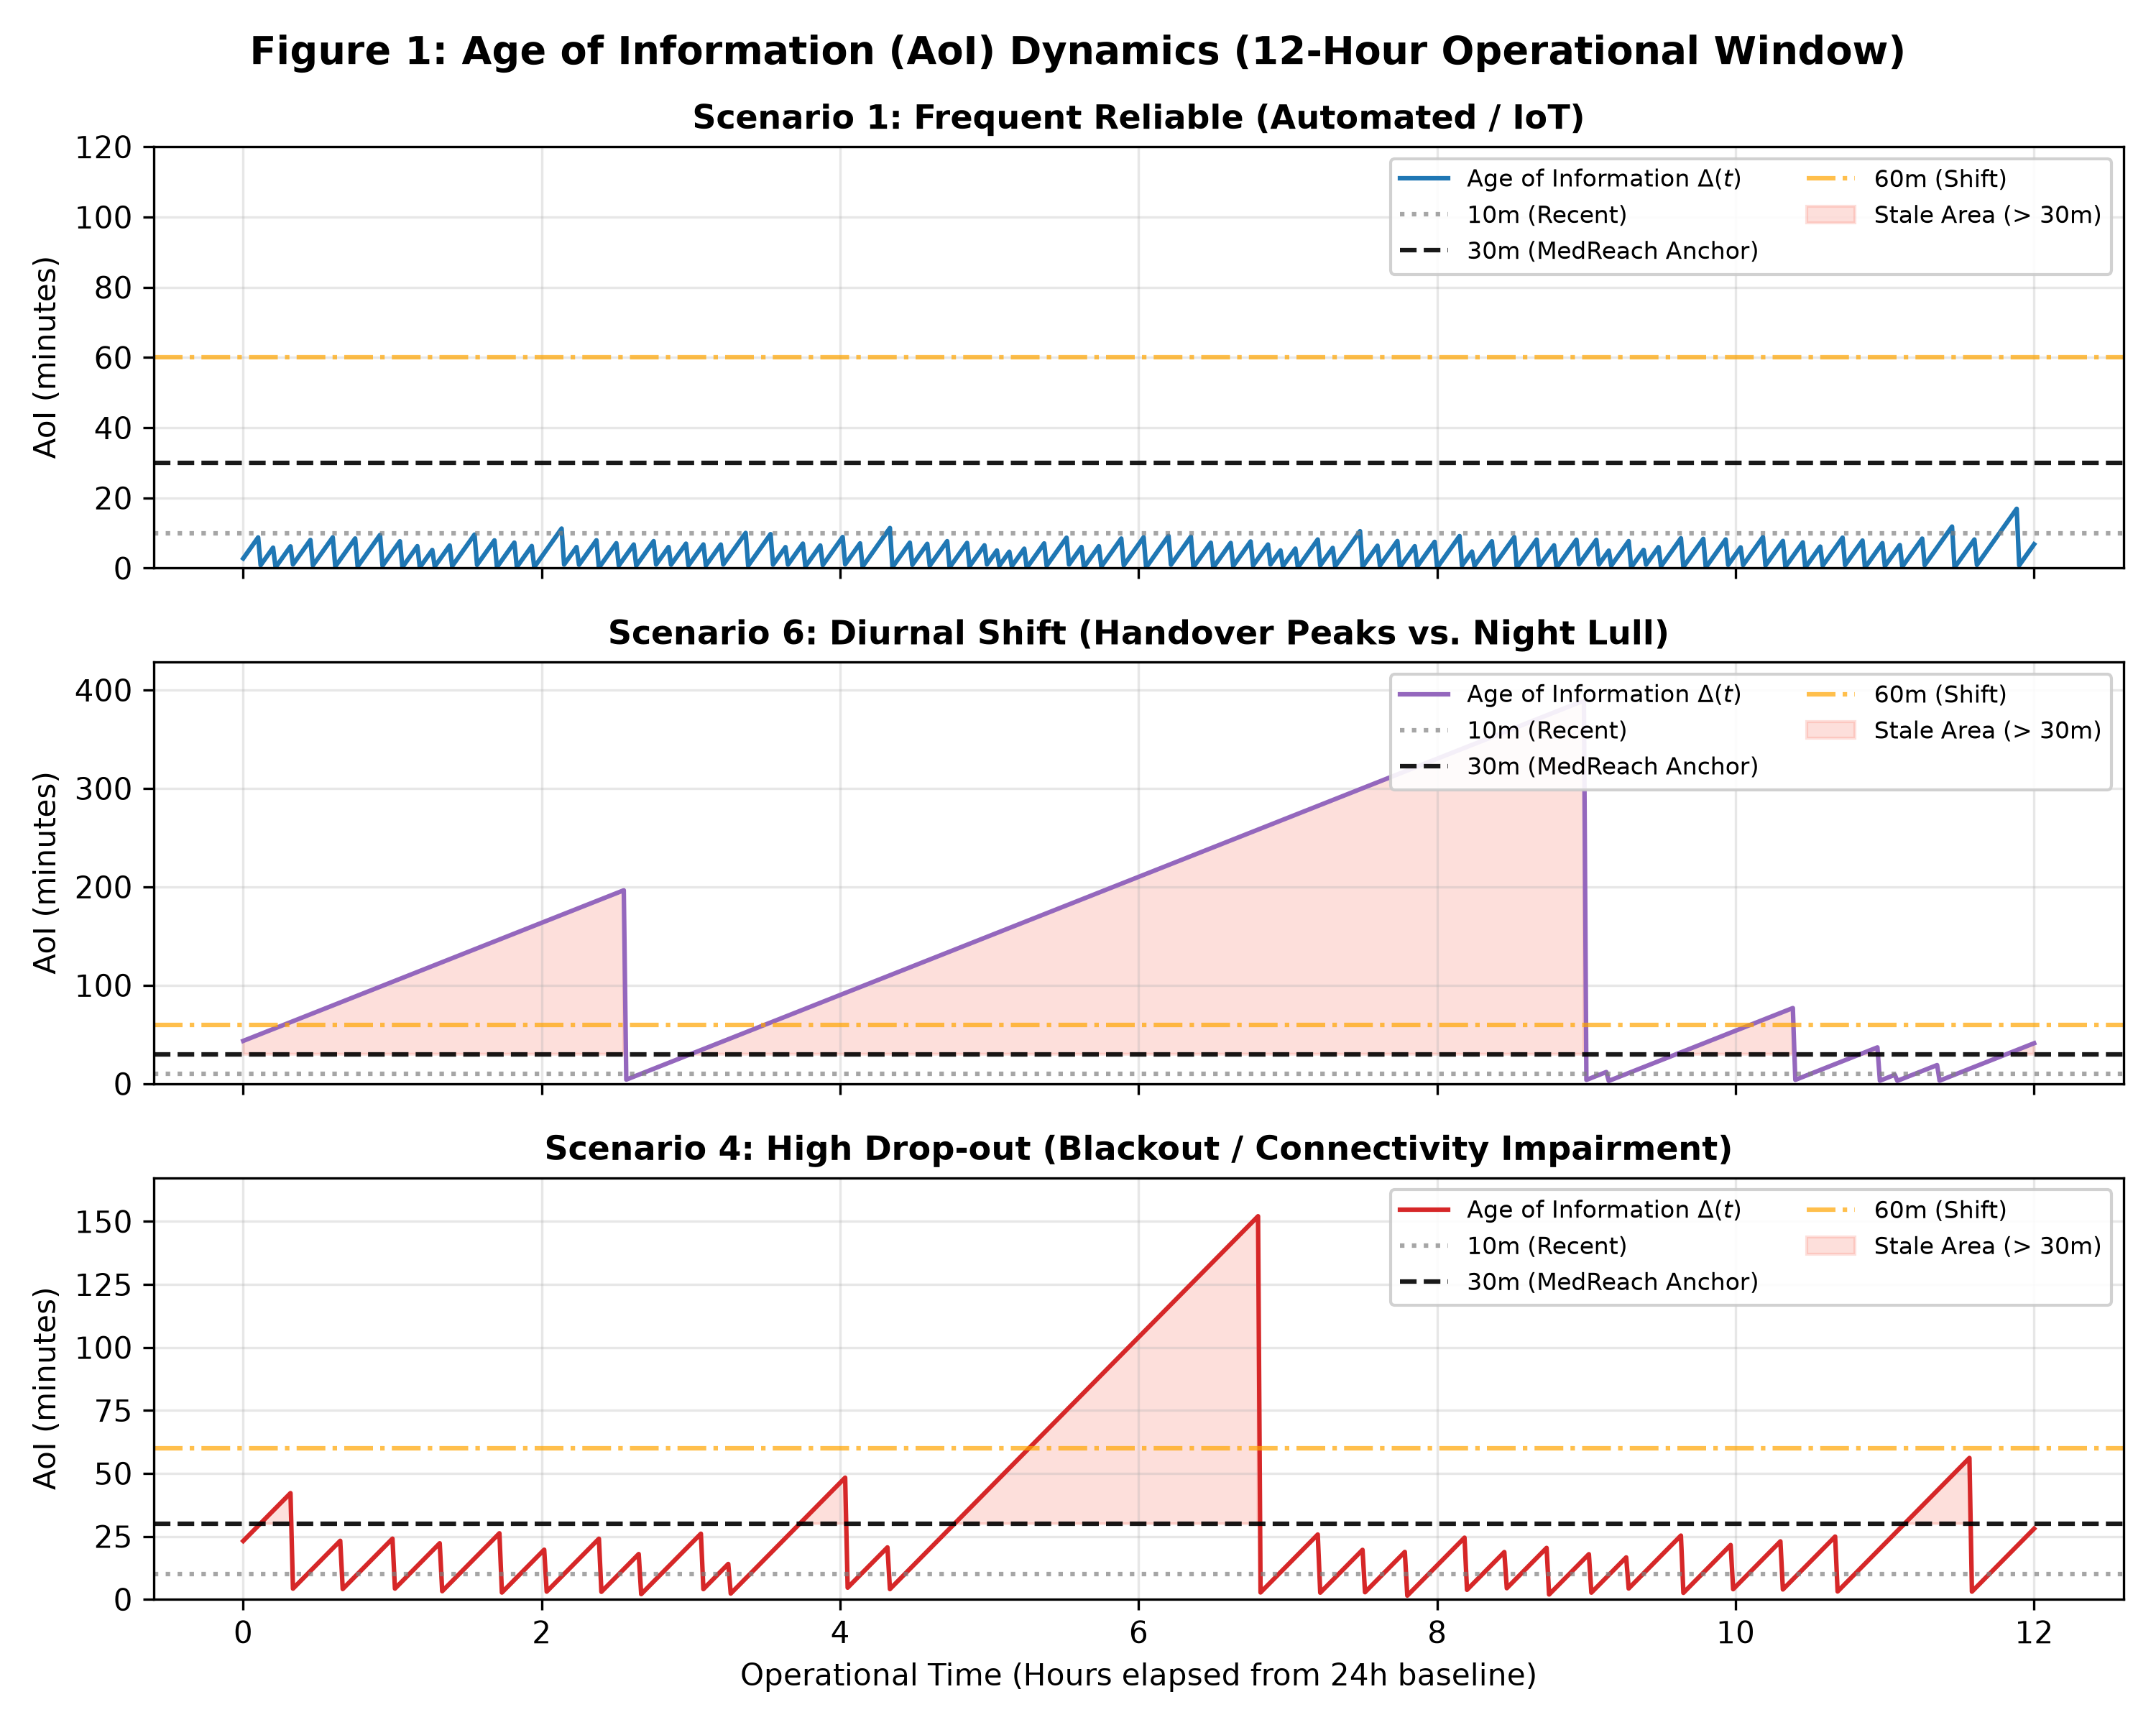
\includegraphics[width=0.98\linewidth]{figures/fig1_aoi_trajectories.png}
\caption{Sample AoI trajectories across operational archetypes.}
\label{fig:aoi_trajectories}
\end{minipage}\hfill
\begin{minipage}{0.48\textwidth}
\centering
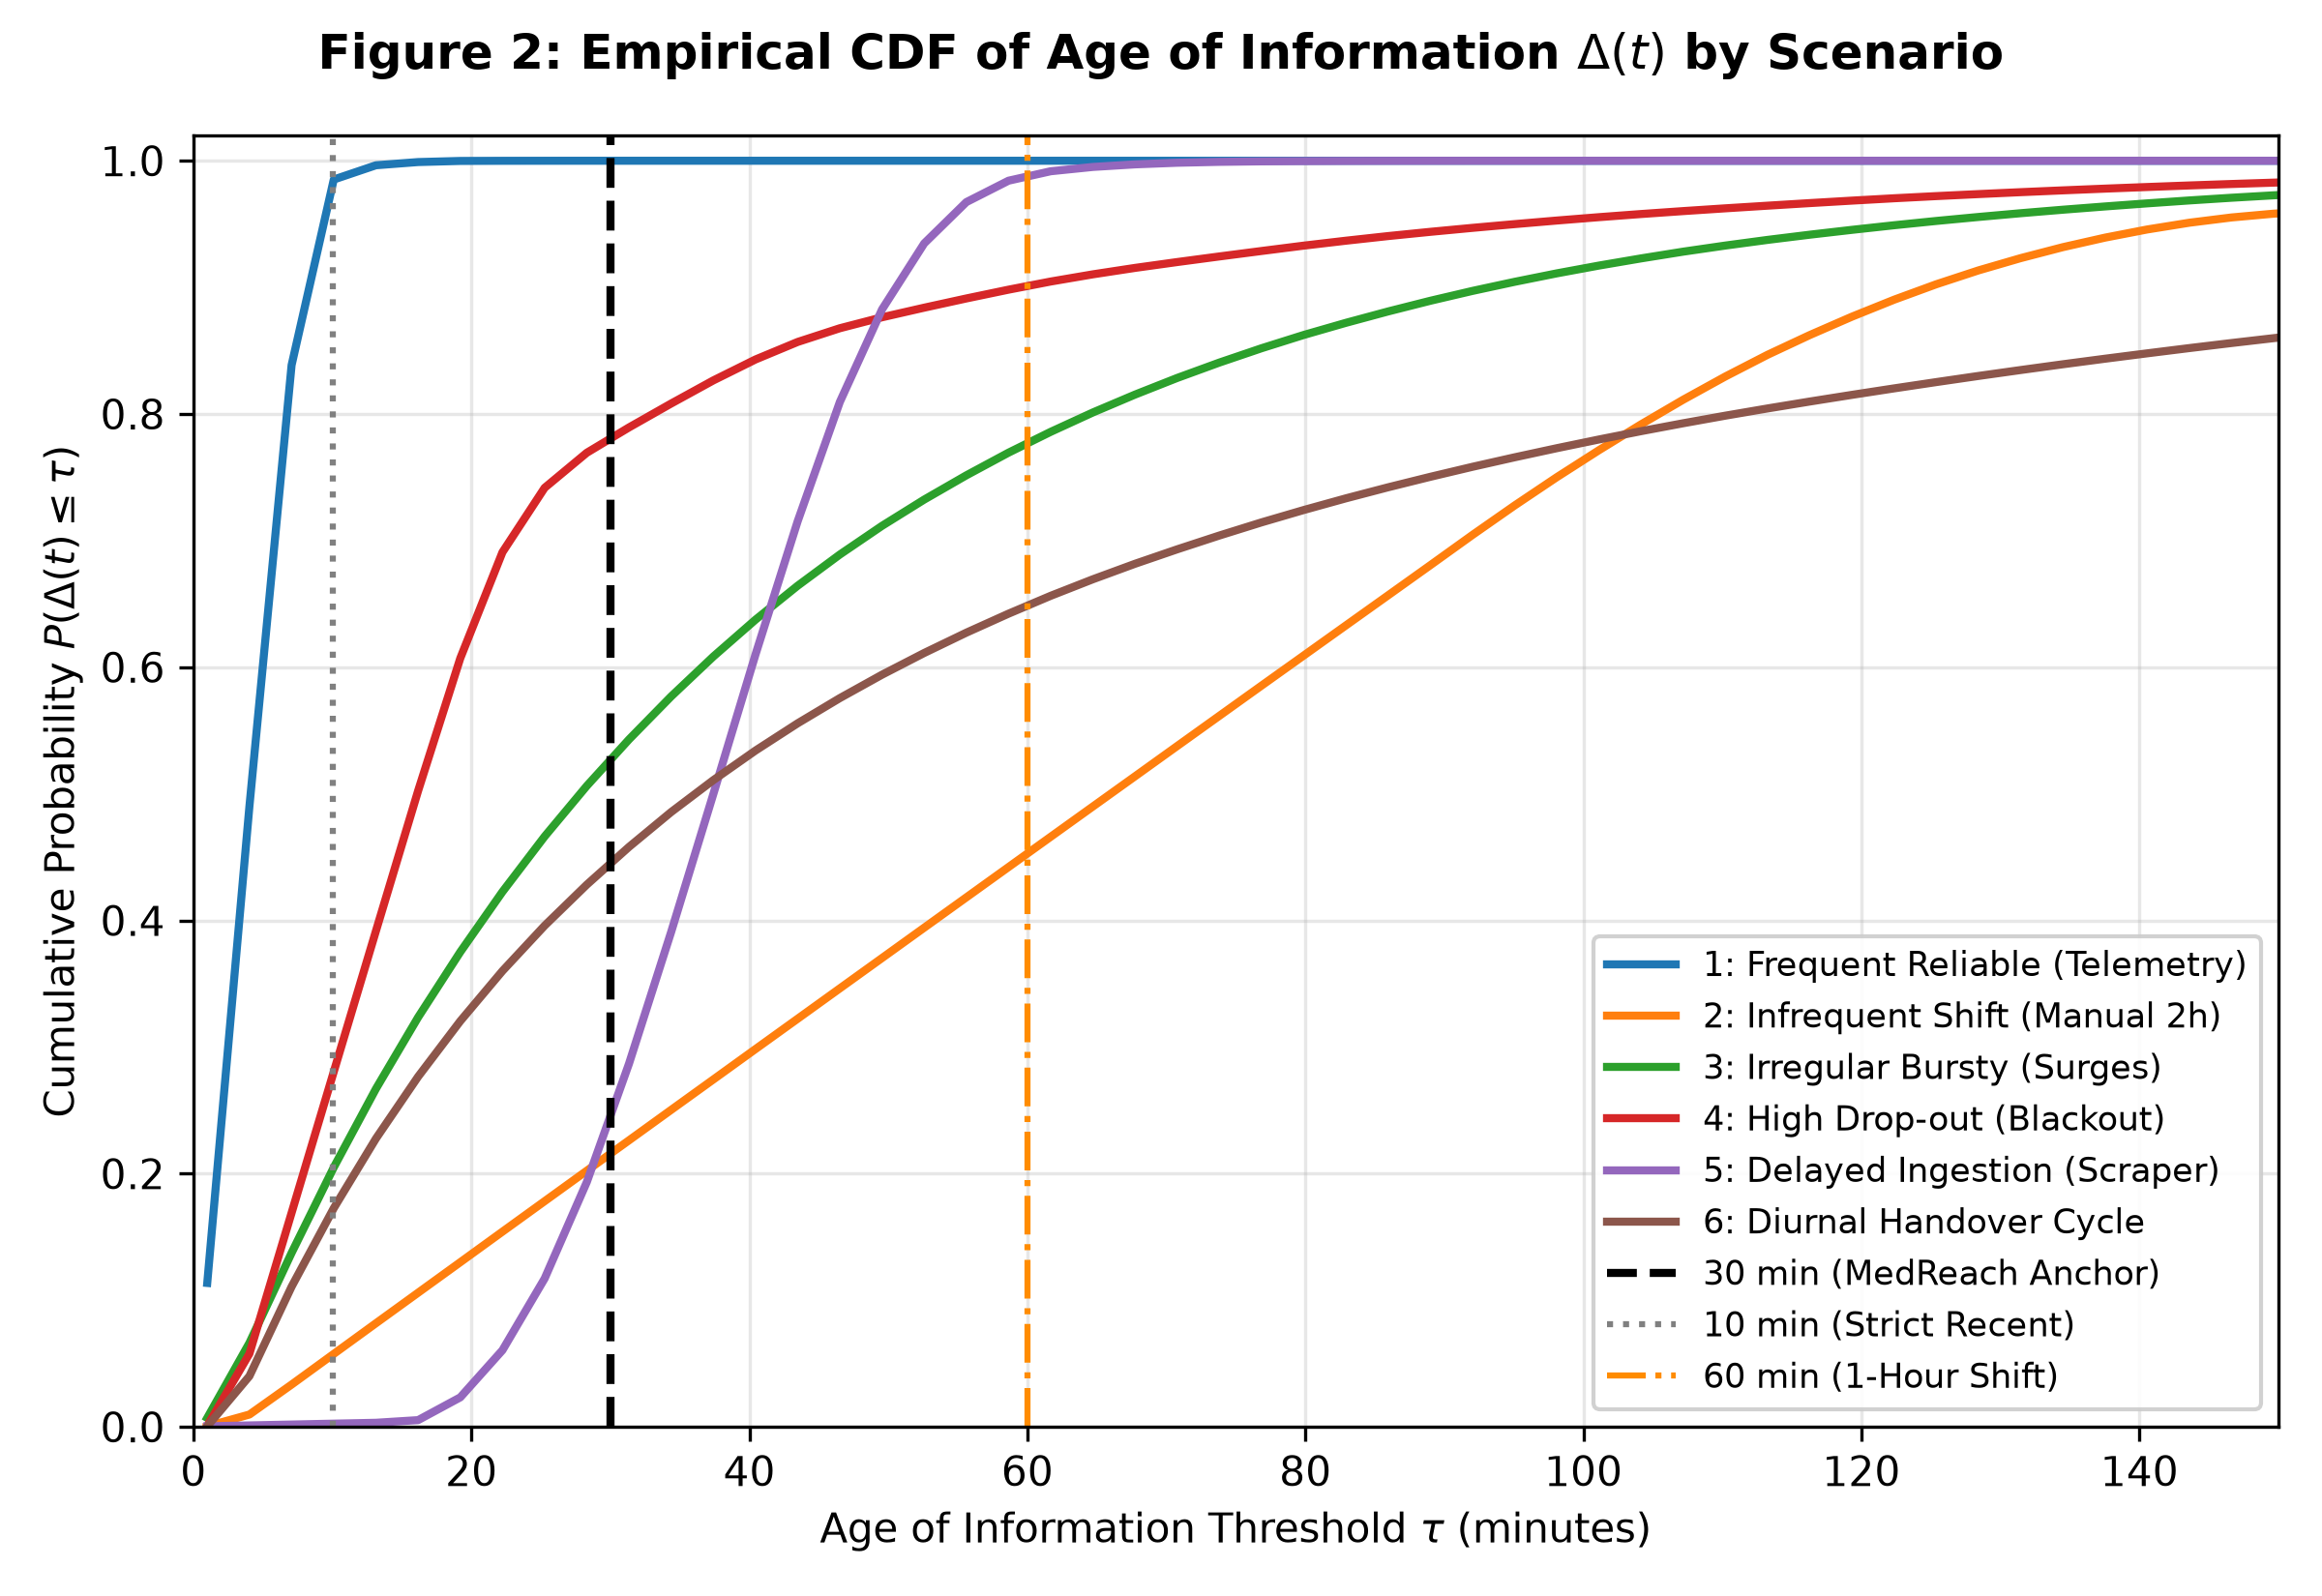
\includegraphics[width=0.98\linewidth]{figures/fig2_aoi_ecdf.png}
\caption{Empirical cumulative distribution of AoI across archetypes.}
\label{fig:aoi_ecdf}
\end{minipage}
\end{figure*}

\begin{figure*}[t]
\centering
\begin{minipage}{0.48\textwidth}
\centering
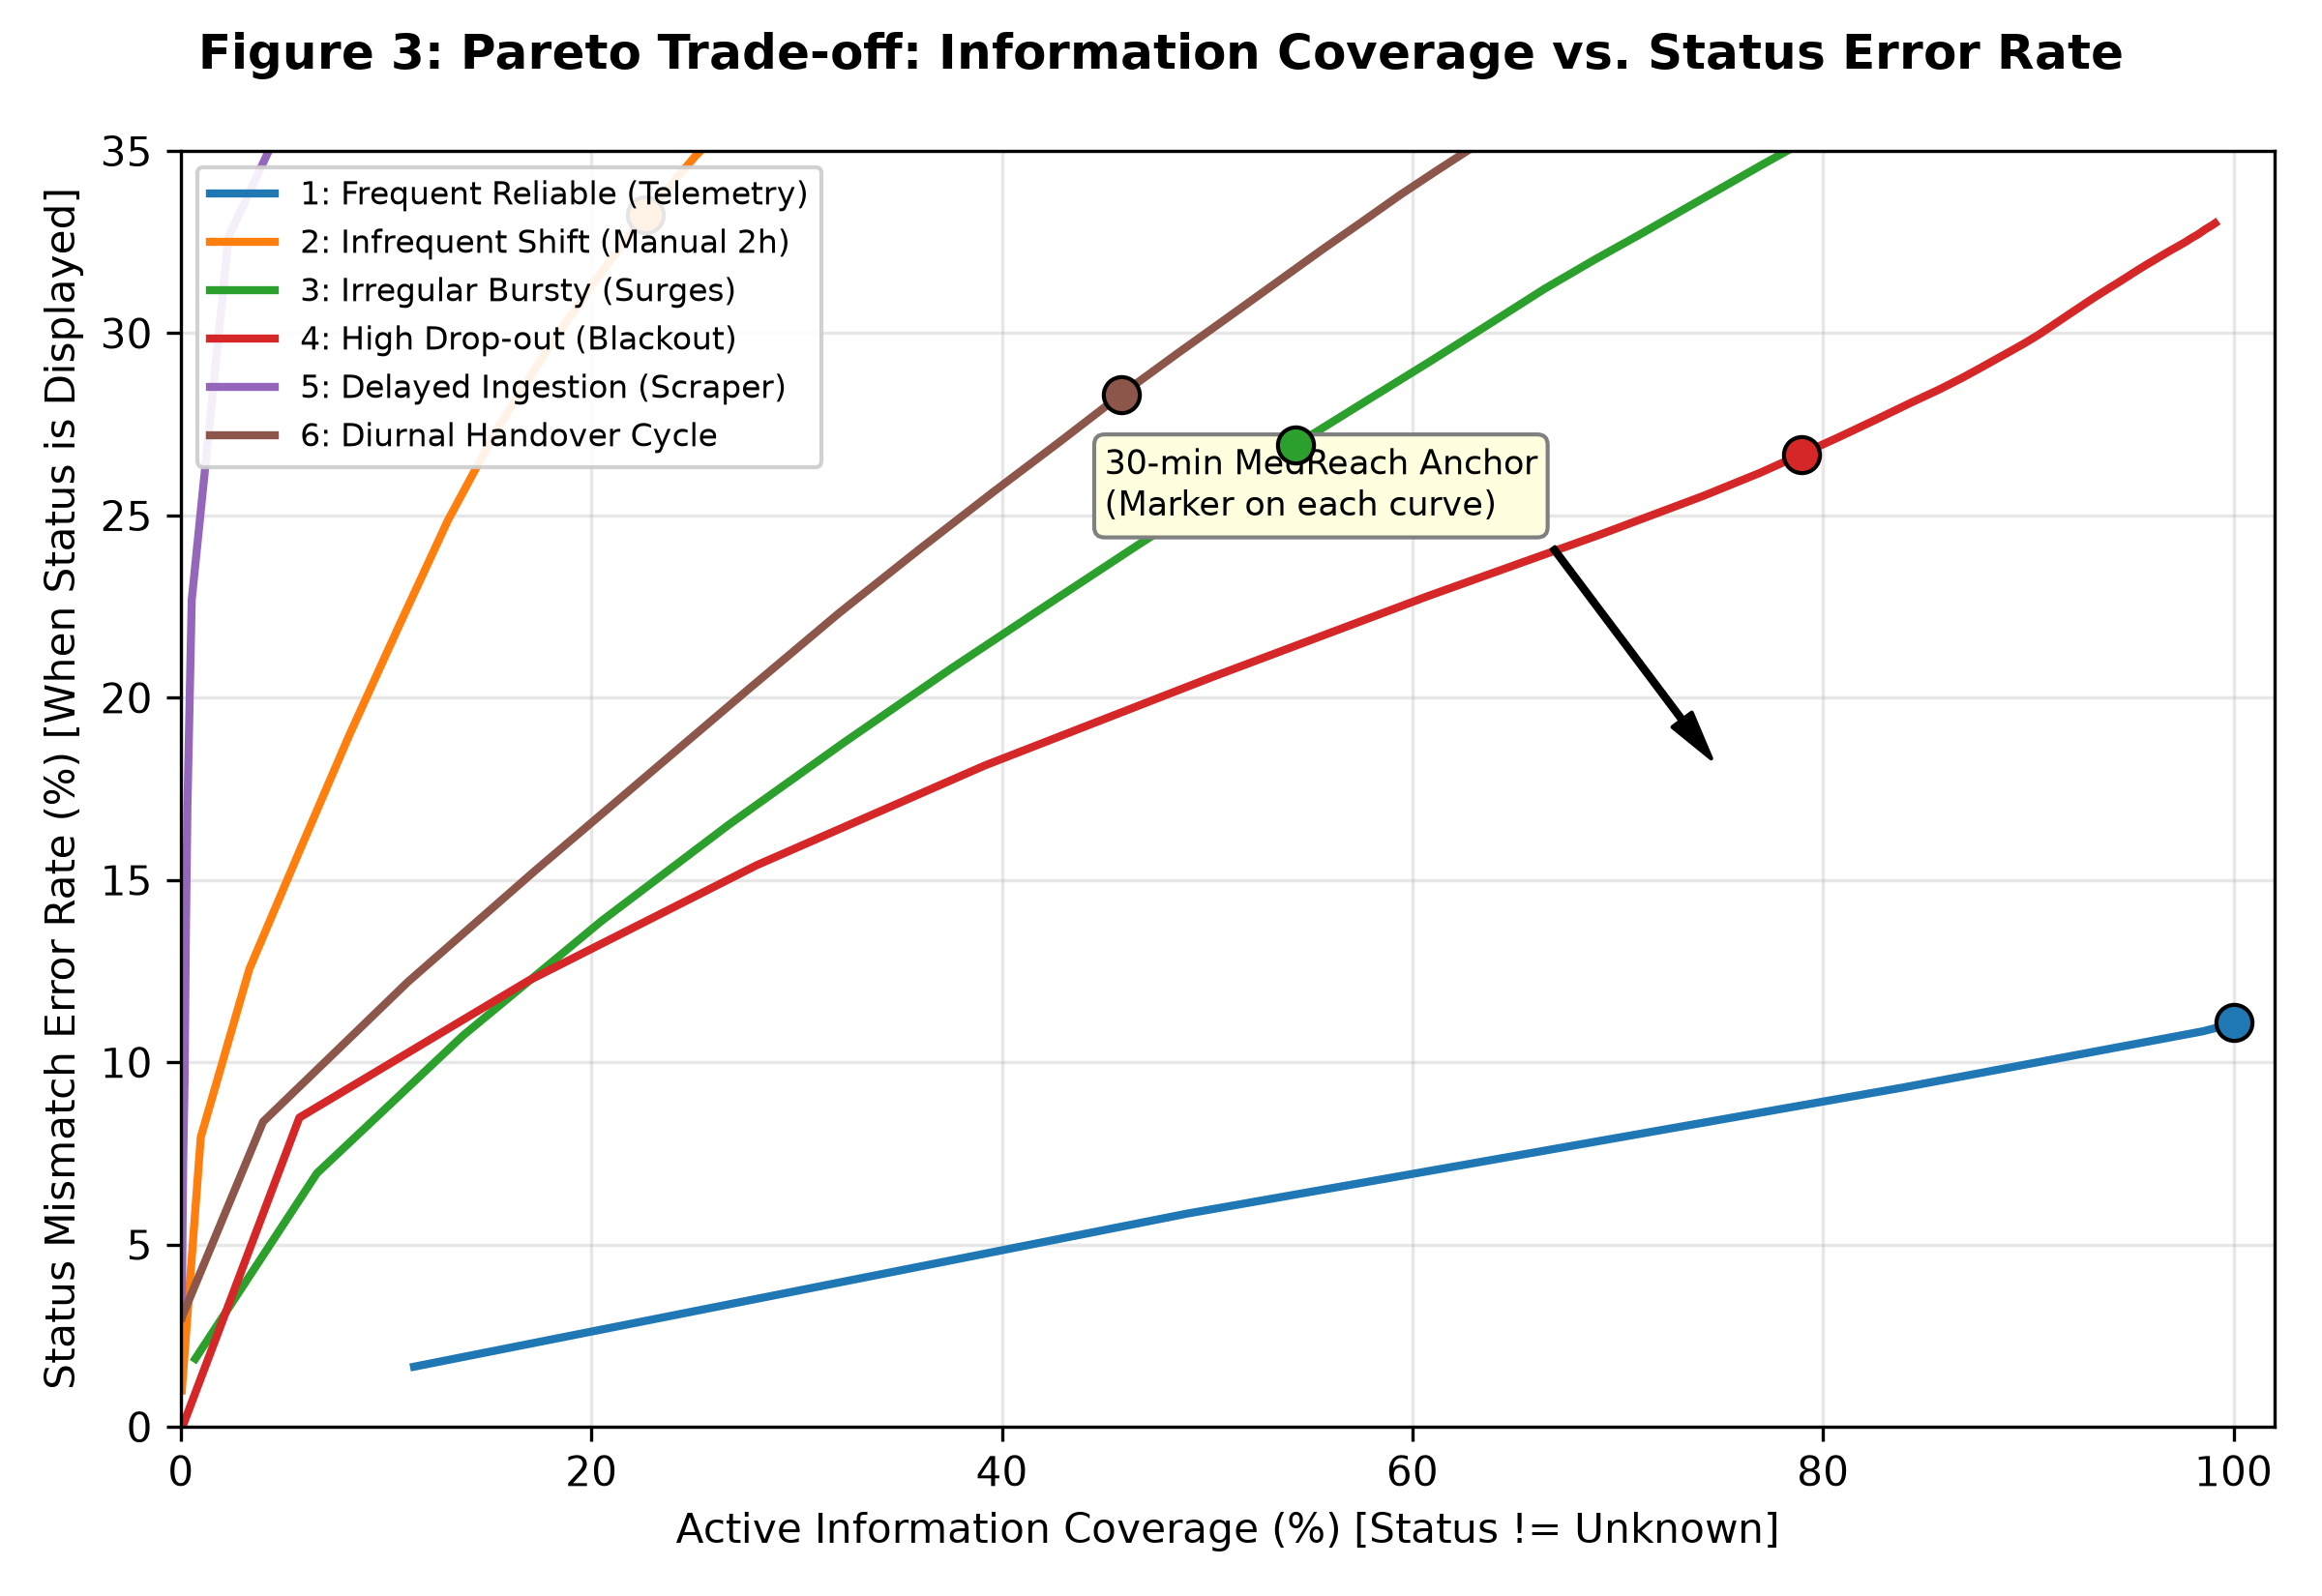
\includegraphics[width=0.98\linewidth]{figures/fig3_error_vs_coverage_pareto.png}
\caption{Pareto trade-off between coverage and status error rate.}
\label{fig:pareto}
\end{minipage}\hfill
\begin{minipage}{0.48\textwidth}
\centering
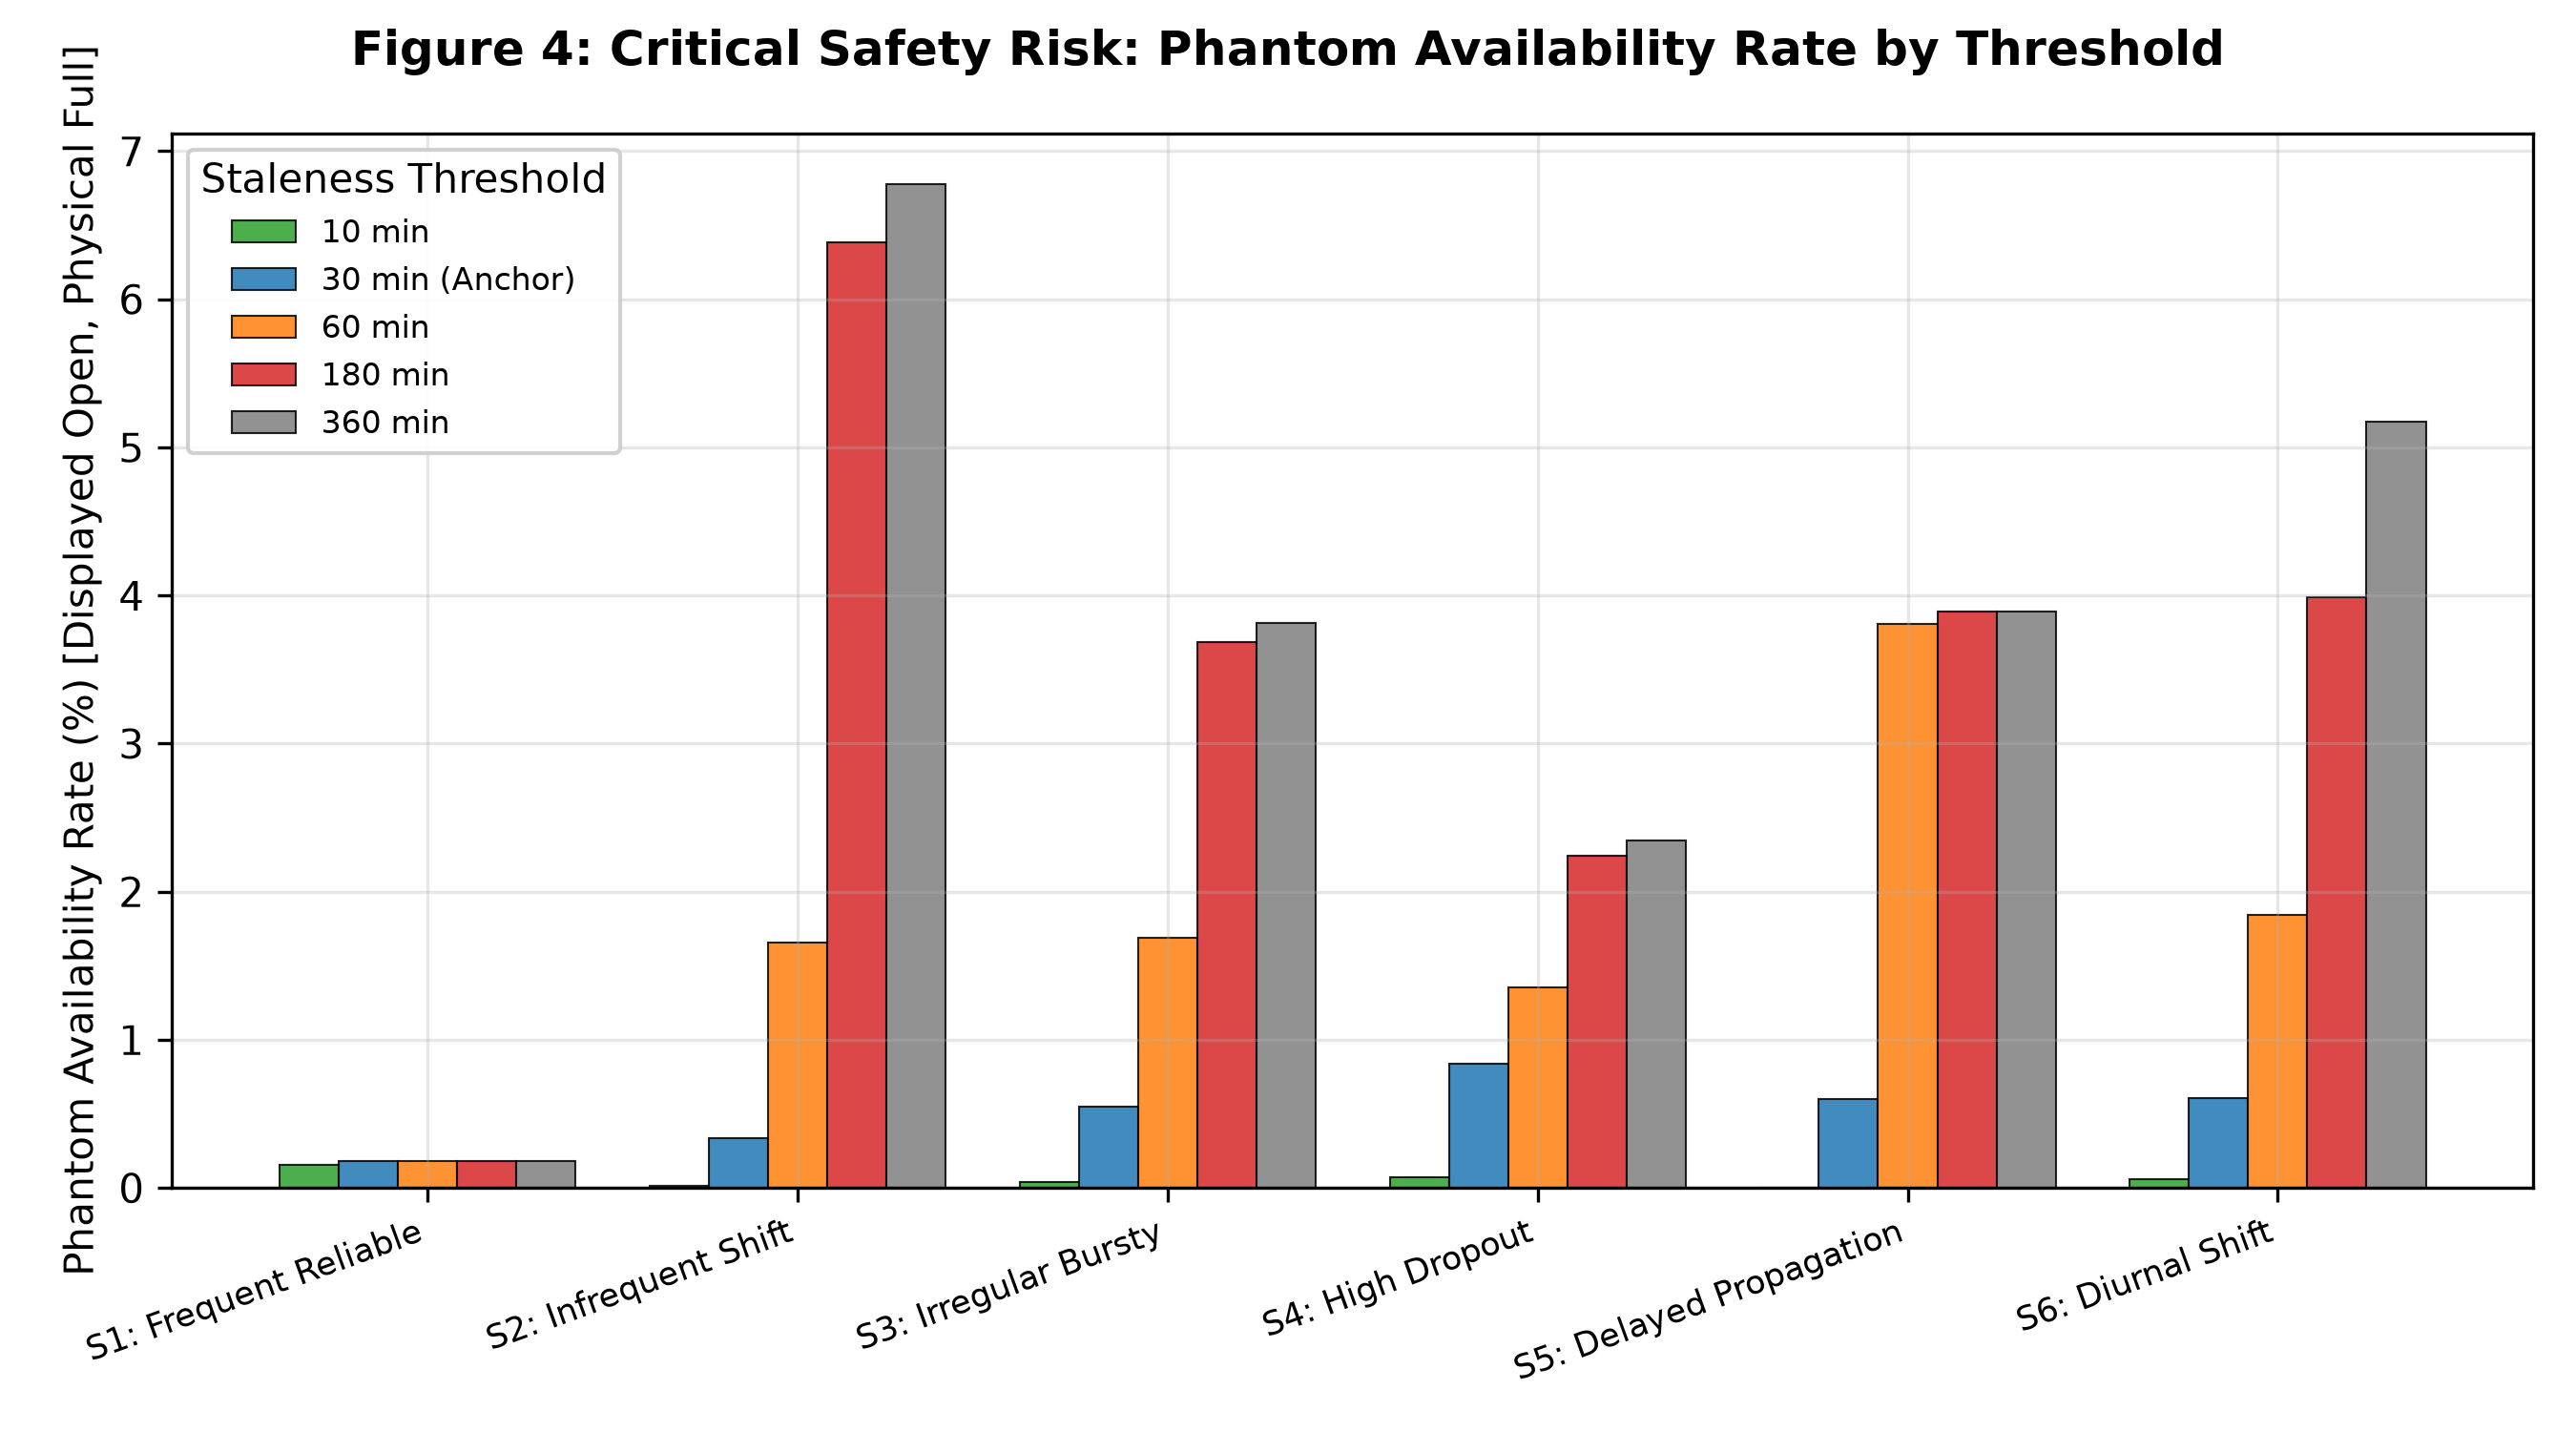
\includegraphics[width=0.98\linewidth]{figures/fig4_phantom_availability_risk.png}
\caption{Phantom availability risk explosion as $\tau$ is relaxed.}
\label{fig:phantom_risk}
\end{minipage}
\end{figure*}

Table~\ref{tab:aoi} summarizes the empirical findings across the 6 operational archetypes under MedReach's pre-registered 30-minute threshold ($\tau = 30\text{ min}$) compared to relaxed thresholds ($\tau = 180\text{ min}$).

\begin{table*}[t]
\centering
\caption{Empirical AoI Dynamics and Staleness Performance Across Six Operational Scenarios}
\label{tab:aoi}
\begin{tabularx}{\textwidth}{X r r r r r r}
\toprule
\textbf{Scenario Archetype} & \textbf{Mean / Med AoI (min)} & \textbf{P95 AoI (min)} & \textbf{Coverage at 30m} & \textbf{Withheld Stale} & \textbf{Error When Known} & \textbf{Phantom Avail (30m vs 180m)} \\
\midrule
S1: Frequent Telemetry & 4.30 / 4.11 & 8.70 & 100.00\% & 0.00\% & 11.10\% & 0.18\% vs 0.18\% \\
S2: Infrequent Shift & 70.51 / 66.10 & 150.31 & 21.58\% & 78.42\% & 32.49\% & 0.34\% vs 6.38\% \\
S3: Irregular Bursty & 40.94 / 27.35 & 125.09 & 52.72\% & 47.28\% & 26.38\% & 0.55\% vs 3.69\% \\
S4: High Dropout & 26.38 / 16.13 & 94.81 & 78.09\% & 21.91\% & 26.46\% & 0.84\% vs 2.25\% \\
S5: Crawler Ingest & 37.50 / 37.55 & 53.76 & 24.39\% & 75.61\% & 41.74\% & 0.60\% vs 3.90\% \\
S6: Diurnal Handover & 73.04 / 35.60 & 281.21 & 44.53\% & 55.47\% & 27.76\% & 0.61\% vs 3.99\% \\
\bottomrule
\end{tabularx}
\end{table*}

The empirical results demonstrate:
\begin{itemize}
    \item \textbf{AoI Trajectories and Information Decay}: As illustrated in Fig.~\ref{fig:aoi_trajectories} and the cumulative distribution functions in Fig.~\ref{fig:aoi_ecdf}, information age grows rapidly under intermittent reporting, requiring deterministic thresholds to prevent stale data dissemination. When balancing coverage against error rate across varying threshold levels (Fig.~\ref{fig:pareto}), MedReach's 30-minute anchor establishes an optimal operational frontier.
    \item \textbf{The Phantom Availability Surge}: Under manual shift reporting (S2), the 30-minute threshold withholds status 78.42\% of the time, keeping phantom availability down to 0.337\%. Relaxing the threshold to $\tau = 180\text{ min}$ expands coverage to 97.15\%, but causes phantom availability to surge by \textbf{18.9$\times$ to 6.382\%}, with overall status error reaching 53.71\% (Fig.~\ref{fig:phantom_risk}).
    \item \textbf{The Ingestion Delay Trap}: In S5, web scrapers scrape data with 15--45 min queue latency. At $\tau = 30\text{ min}$, \textbf{51.79\% of updates arrive already stale}. If the threshold is tightened to $\tau = 10\text{ min}$, \textbf{99.64\% arrive already stale}, driving active coverage down to 0.25\%. This proves that discovery freshness is strictly bounded by ingestion delay.
\end{itemize}

\subsection{RQ2: Multi-Source Provenance and Conflicting-Claim Fusion (EXP-PROV)}

\begin{figure*}[t]
\centering
\begin{minipage}{0.48\textwidth}
\centering
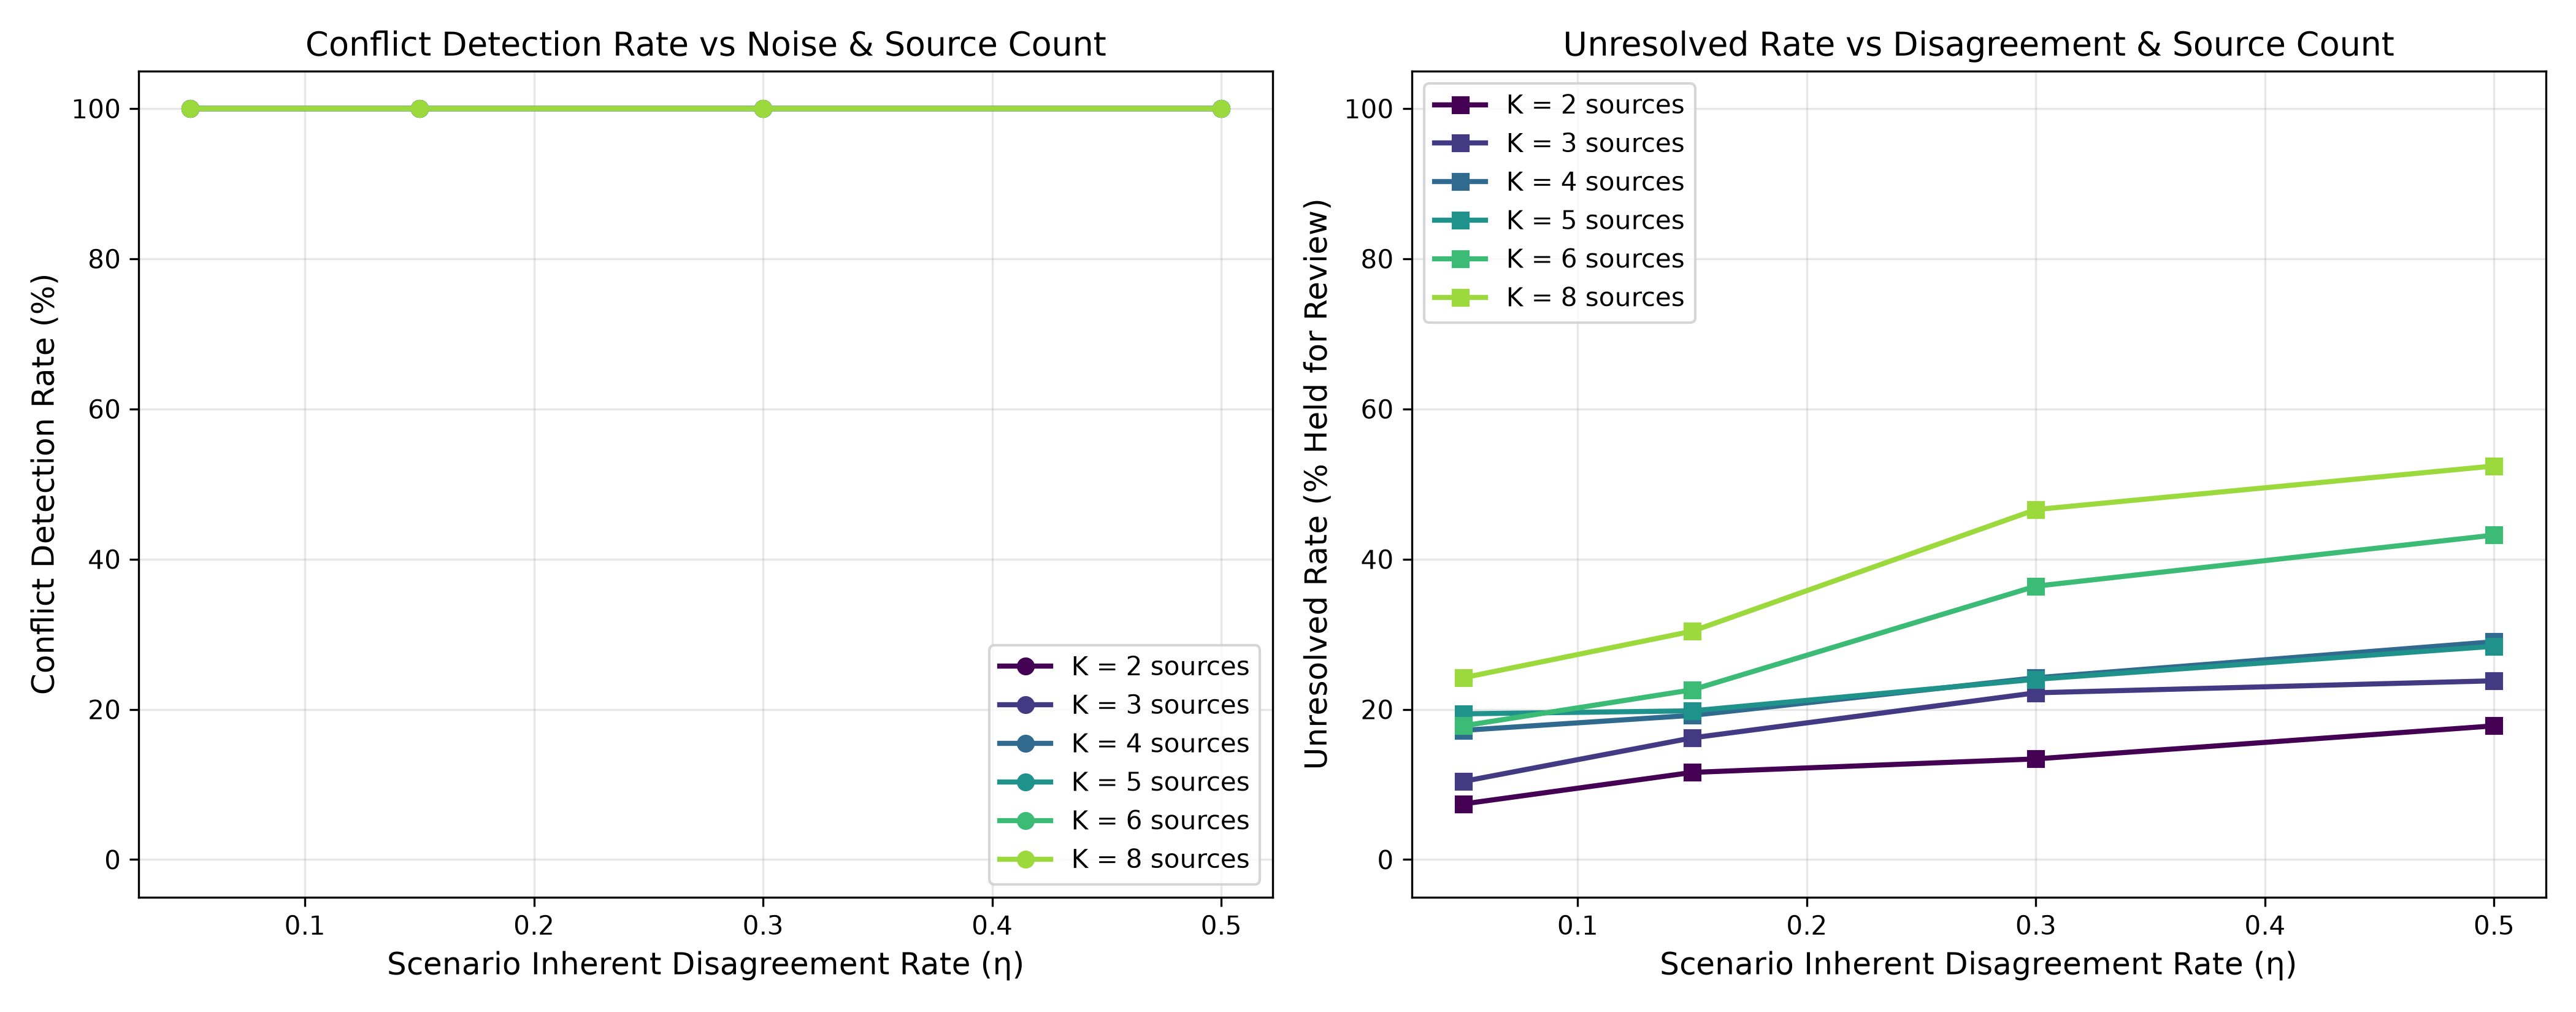
\includegraphics[width=0.95\linewidth]{figures/fig1_conflict_detection.png}
\caption{Conflict detection and fallback rates across source disagreement rates.}
\label{fig:fusion_conflict}
\end{minipage}\hfill
\begin{minipage}{0.48\textwidth}
\centering
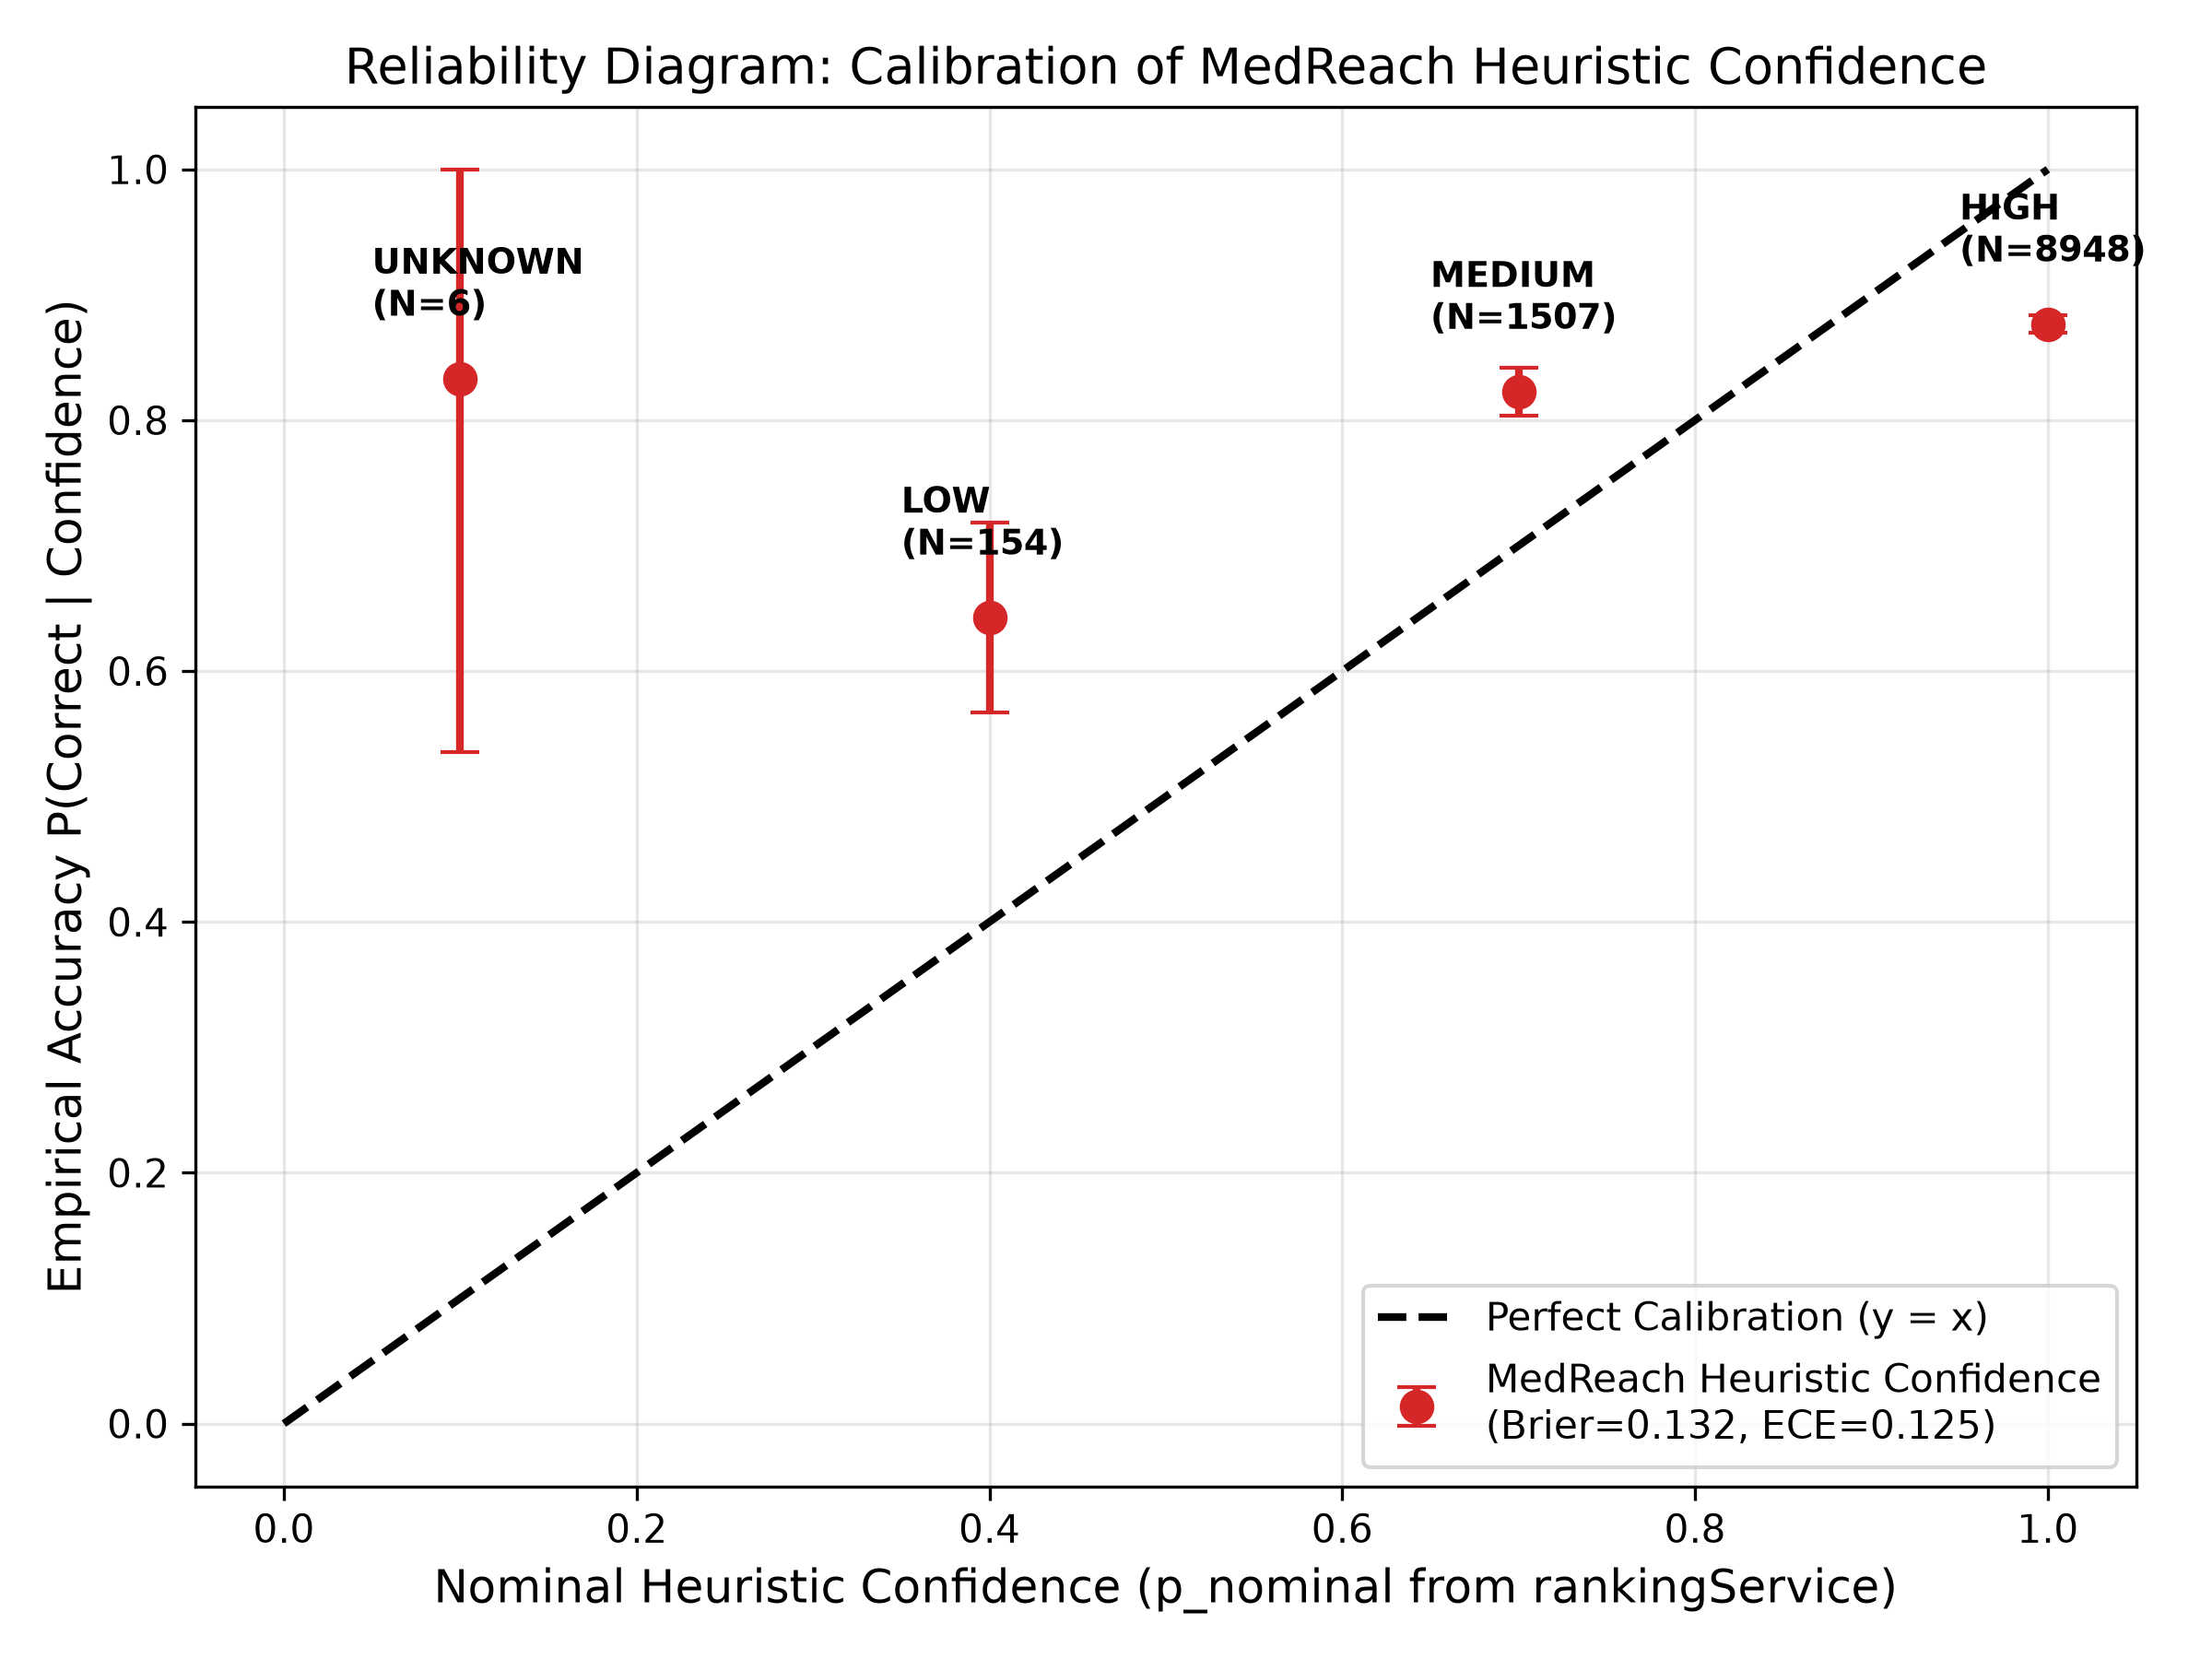
\includegraphics[width=0.95\linewidth]{figures/fig5_calibration_curve.png}
\caption{Reliability calibration curve showing heuristic confidence vs accuracy.}
\label{fig:calibration_curve}
\end{minipage}
\end{figure*}

Evaluating 40,000+ synthetic trials established:
\begin{itemize}
    \item \textbf{100.0\% Conflict Detection}: Divergent claims across facility capabilities and structured attributes are universally detected. As illustrated in Fig.~\ref{fig:fusion_conflict}, the cascade consistently isolates unverified conflicting reports as source disagreement increases.
    \item \textbf{Conservative Ignorance Fallback}: Under unverified scraper conflicts, the engine safely held the status as \texttt{unknown} in \textbf{87.1\%} of cases. When verified official anchors exist, the engine achieved \textbf{95.9\% correct resolution} and 0.0\% decision error.
    \item \textbf{Conditional Accuracy}: Across 12,000 trials with known ground truth, when a claim was resolved, the engine achieved \textbf{90.29\% conditional accuracy} (overall decision error rate 7.38\%).
\end{itemize}

\begin{table}[ht]
\centering
\caption{Heuristic Confidence Calibration Analysis (EXP-PROV-05)}
\label{tab:calibration}
\begin{tabularx}{\linewidth}{l r r r r}
\toprule
\textbf{Label} & \textbf{Nominal $P$} & \textbf{Samples} & \textbf{Accuracy} & \textbf{95\% CI} \\
\midrule
HIGH & 1.000 & 8,948 & 0.8765 & [0.8697, 0.8833] \\
MEDIUM & 0.700 & 1,507 & 0.8228 & [0.8035, 0.8421] \\
LOW & 0.400 & 154 & 0.6429 & [0.5672, 0.7185] \\
UNKNOWN & 0.100 & 6 & 0.8333 & [0.5351, 1.0000] \\
\bottomrule
\end{tabularx}
\end{table}

\textbf{Critical Negative Finding}: As shown in Table~\ref{tab:calibration} and Fig.~\ref{fig:calibration_curve}, formal calibration analysis reveals that MedReach's confidence score is an \textbf{uncalibrated heuristic ranking} rather than a calibrated probability:
\begin{itemize}
    \item Brier Score: \textbf{0.1315}
    \item Expected Calibration Error (ECE): \textbf{0.1255}
    \item Maximum Calibration Error (MCE): \textbf{0.7333}
    \item Verdict: \texttt{UNBOUNDED\_HEURISTIC\_RANKING}
\end{itemize}
The score represents an ordinal source-prioritization weight, not a statistical confidence probability.

\subsection{RQ3: Data Path \& Edge Caching Staleness Audit (EXP-DATAPATH)}
\textbf{Definitive Verdict: NOT SUPPORTED}.
An architectural audit of 22 deployed endpoints across Vercel and Railway refuted an earlier theoretical concern:
\begin{itemize}
    \item \textbf{Zero Volatile Data in HTML Shells}: Edge-cached HTML shells served with \texttt{x-vercel-cache: HIT} (age ~32,000s) contain only static structural skeletons, navigation bars, and placeholder text (``Loading providers...''). They contain \textbf{zero} clinical availability counts, bed numbers, or provider database records.
    \item \textbf{Universal Client-Side Runtime Fetching}: All 15 discovery and emergency routes enforce \texttt{"use client";} directives. Data fetching occurs strictly in React \texttt{useEffect} hooks \textit{after} DOM hydration.
    \item \textbf{Independent Backend Header Policy}: The Express backend operates on Railway, emitting \texttt{Cache-Control: no-store} on all transactional endpoints.
\end{itemize}
Thus, edge caching of static HTML shells does not induce healthcare availability staling.

\subsection{RQ4: Transactional Reliability \& State-Machine Invariants (EXP-TX)}
In the master transactional reliability suite, MedReach achieved a \textbf{100.0\% pass rate (48 passed / 0 failed)}, as shown in Table~\ref{tab:transactional}.

\begin{table}[ht]
\centering
\caption{Transactional Reliability \& Concurrency Suite Results (EXP-TX)}
\label{tab:transactional}
\begin{tabularx}{\linewidth}{l p{4.6cm} r r}
\toprule
\textbf{ID} & \textbf{Scenario Evaluated} & \textbf{Tests} & \textbf{Pass\%} \\
\midrule
TX-01 & Duplicate Prevention \& Scoped Idempotency Keys & 10 & 100\% \\
TX-02 & Idempotent Retries \& Timeout Recovery & 5 & 100\% \\
TX-03 & Concurrent Requests Competing for State (OCC) & 5 & 100\% \\
TX-04 & Stale-State \& Out-of-Order Transition Prevention & 6 & 100\% \\
TX-05 & State Machine RBAC \& Role Permissions & 5 & 100\% \\
TX-06 & Interrupted In-Flight Operations \& Resumption & 4 & 100\% \\
TX-07 & Read Consistency During Concurrent Writes & 4 & 100\% \\
TX-08 & Complete Telemetry-Request Decoupling Ledger & 6 & 100\% \\
\midrule
\textbf{TOTAL} & \textbf{Master Transactional Suite} & \textbf{48} & \textbf{100.00\%} \\
\bottomrule
\end{tabularx}
\end{table}

Key guarantees proven:
\begin{enumerate}
    \item Re-submitting an identical key by the same actor returns \texttt{200 OK} with the original document; cross-user reuse is rejected with \texttt{409 IDEMPOTENCY\_KEY\_REUSED}.
    \item Under 10-way simultaneous conflicting state transitions, exactly 1 atomic update commits, and 9 receive \texttt{409 Conflict}.
    \item In EXP-TX-08, submitting 10 emergency requests, accepting 3, and completing 2 did NOT decrement reported availability in \texttt{AvailabilityObservation} (remained 5 beds), proving complete architectural decoupling.
\end{enumerate}

\subsection{RQ5: Isolated Load, Stress, and Recovery Benchmarks (EXP-LOAD)}
\textit{Scope Characterization: These empirical measurements characterize a single local machine operating across loopback networking (\texttt{127.0.0.1}), establishing relative architectural scaling properties rather than distributed cloud capacity.}

\begin{figure*}[t]
\centering
\begin{minipage}{0.48\textwidth}
\centering
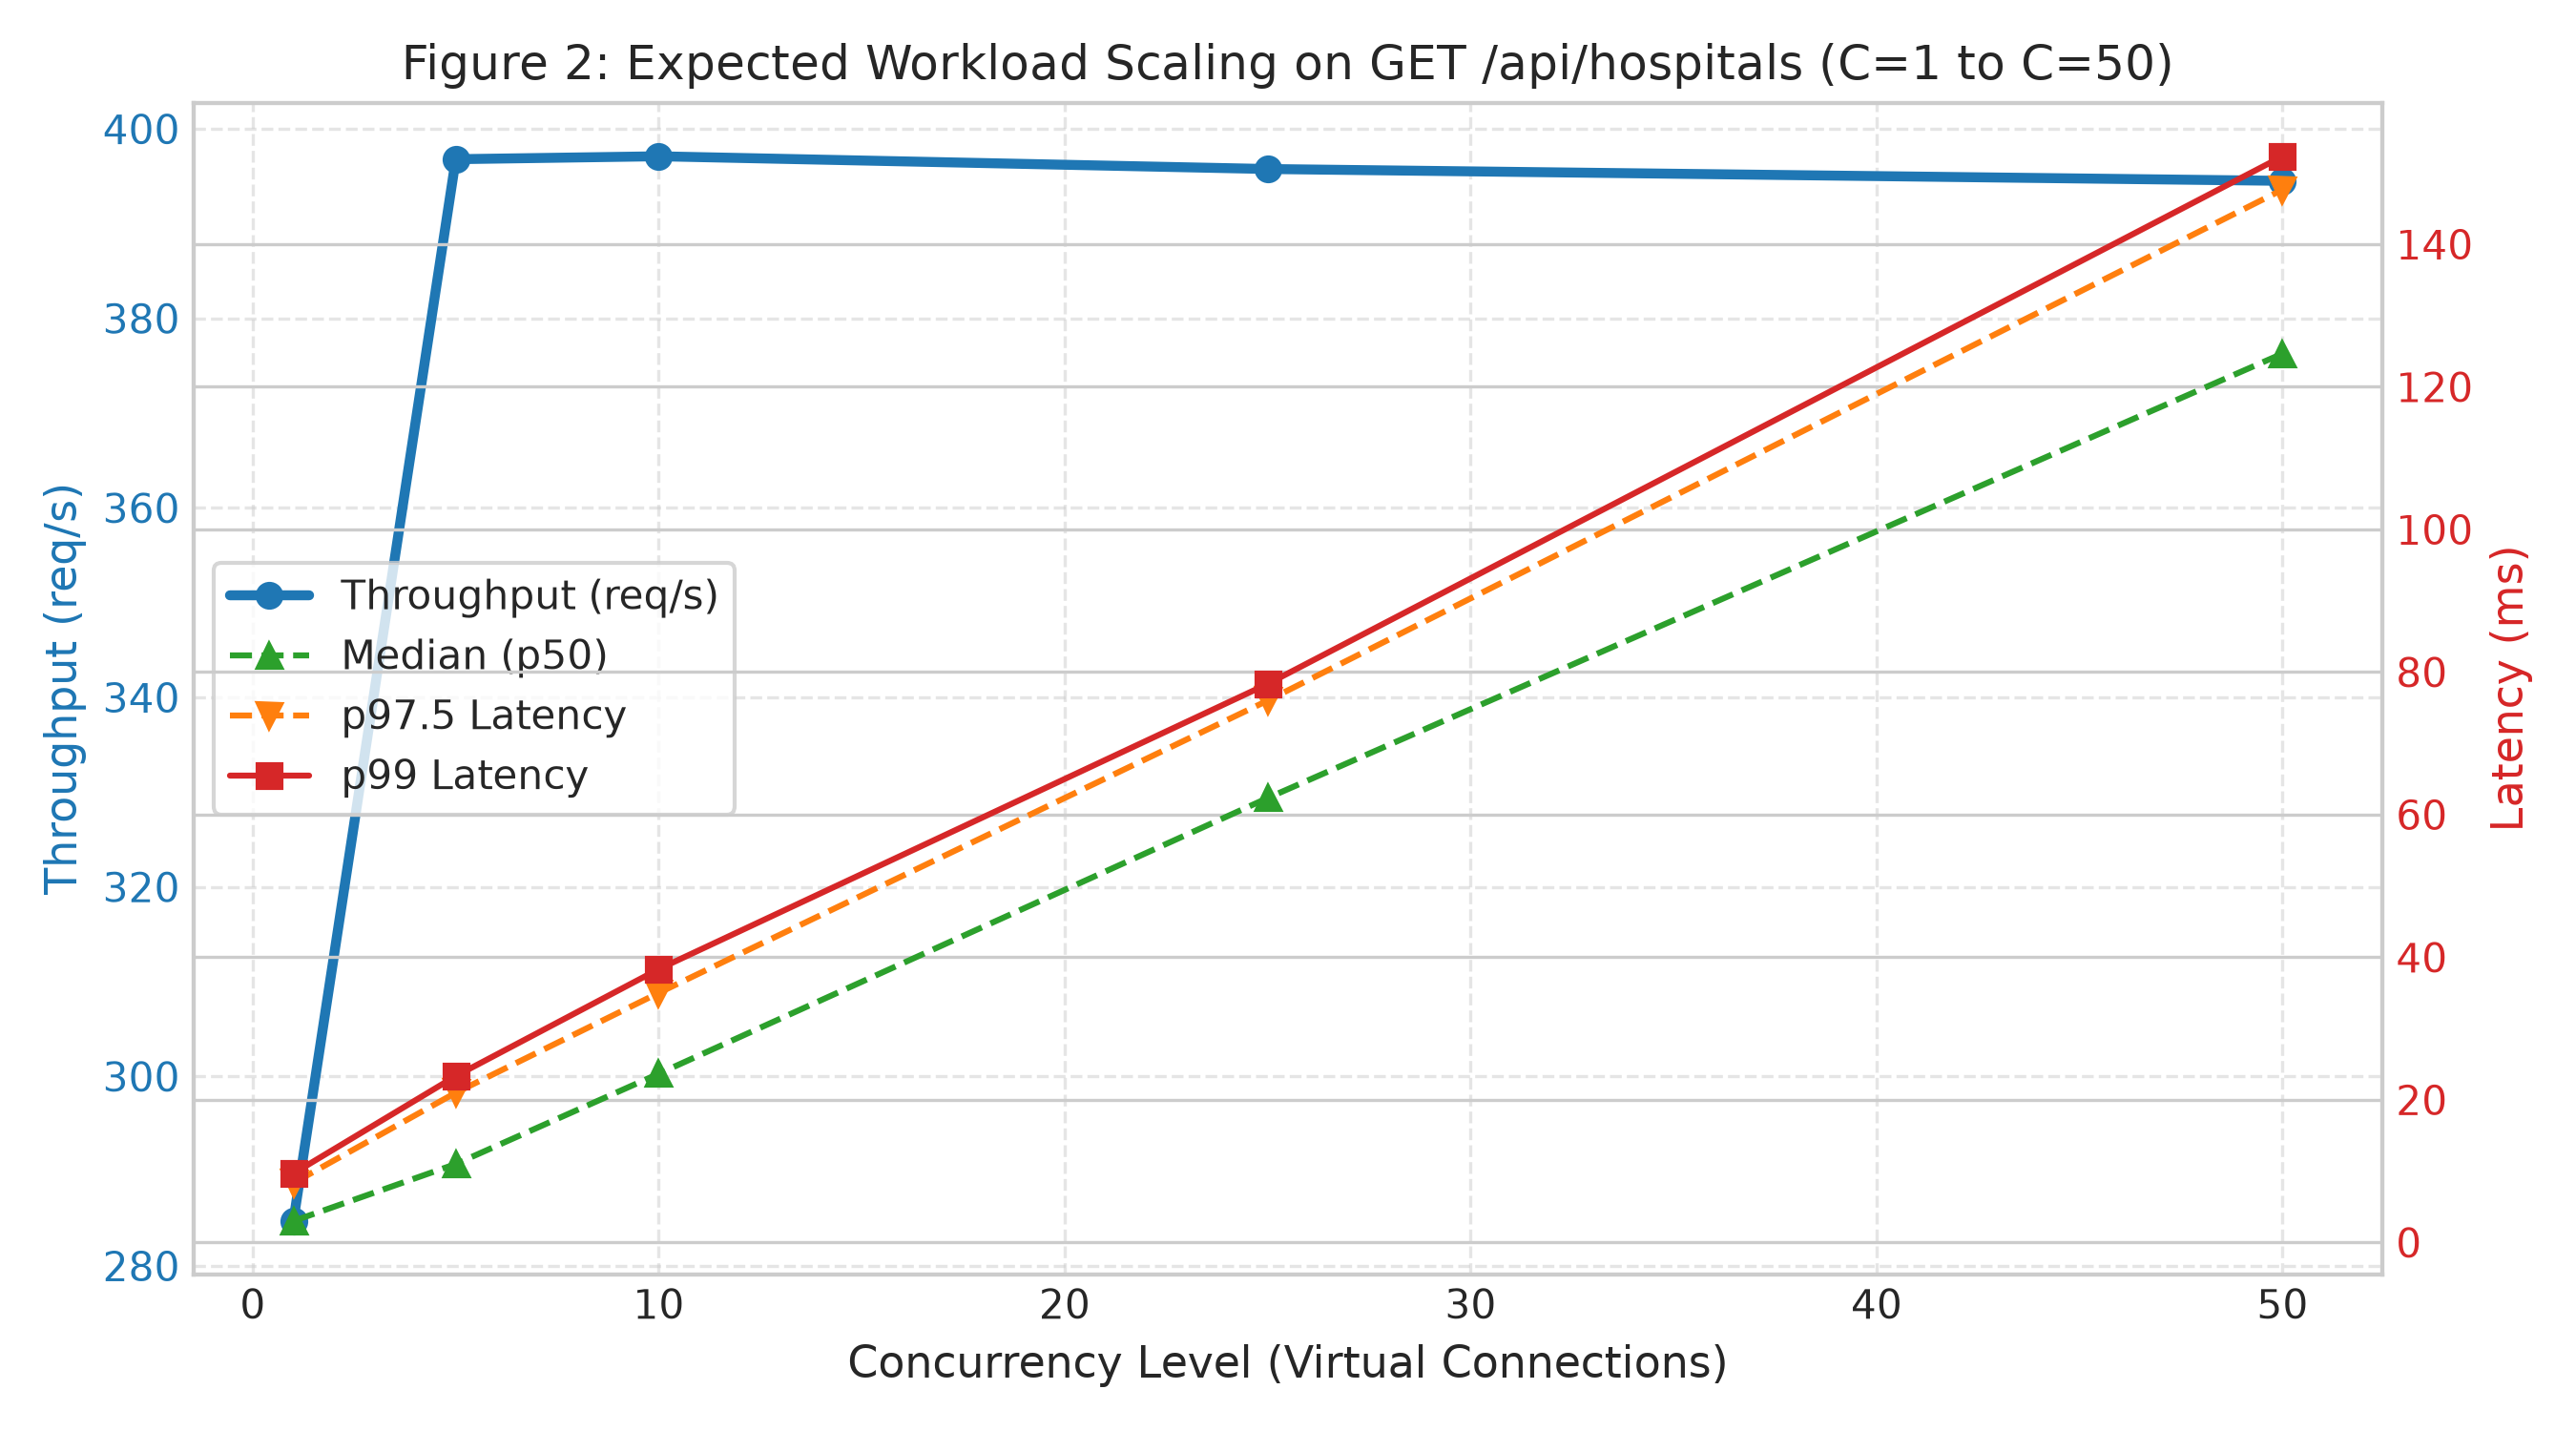
\includegraphics[width=0.98\linewidth]{figures/figure2_workload_scaling.png}
\caption{Throughput scaling and saturation knee on database reads.}
\label{fig:load_scaling}
\end{minipage}\hfill
\begin{minipage}{0.48\textwidth}
\centering
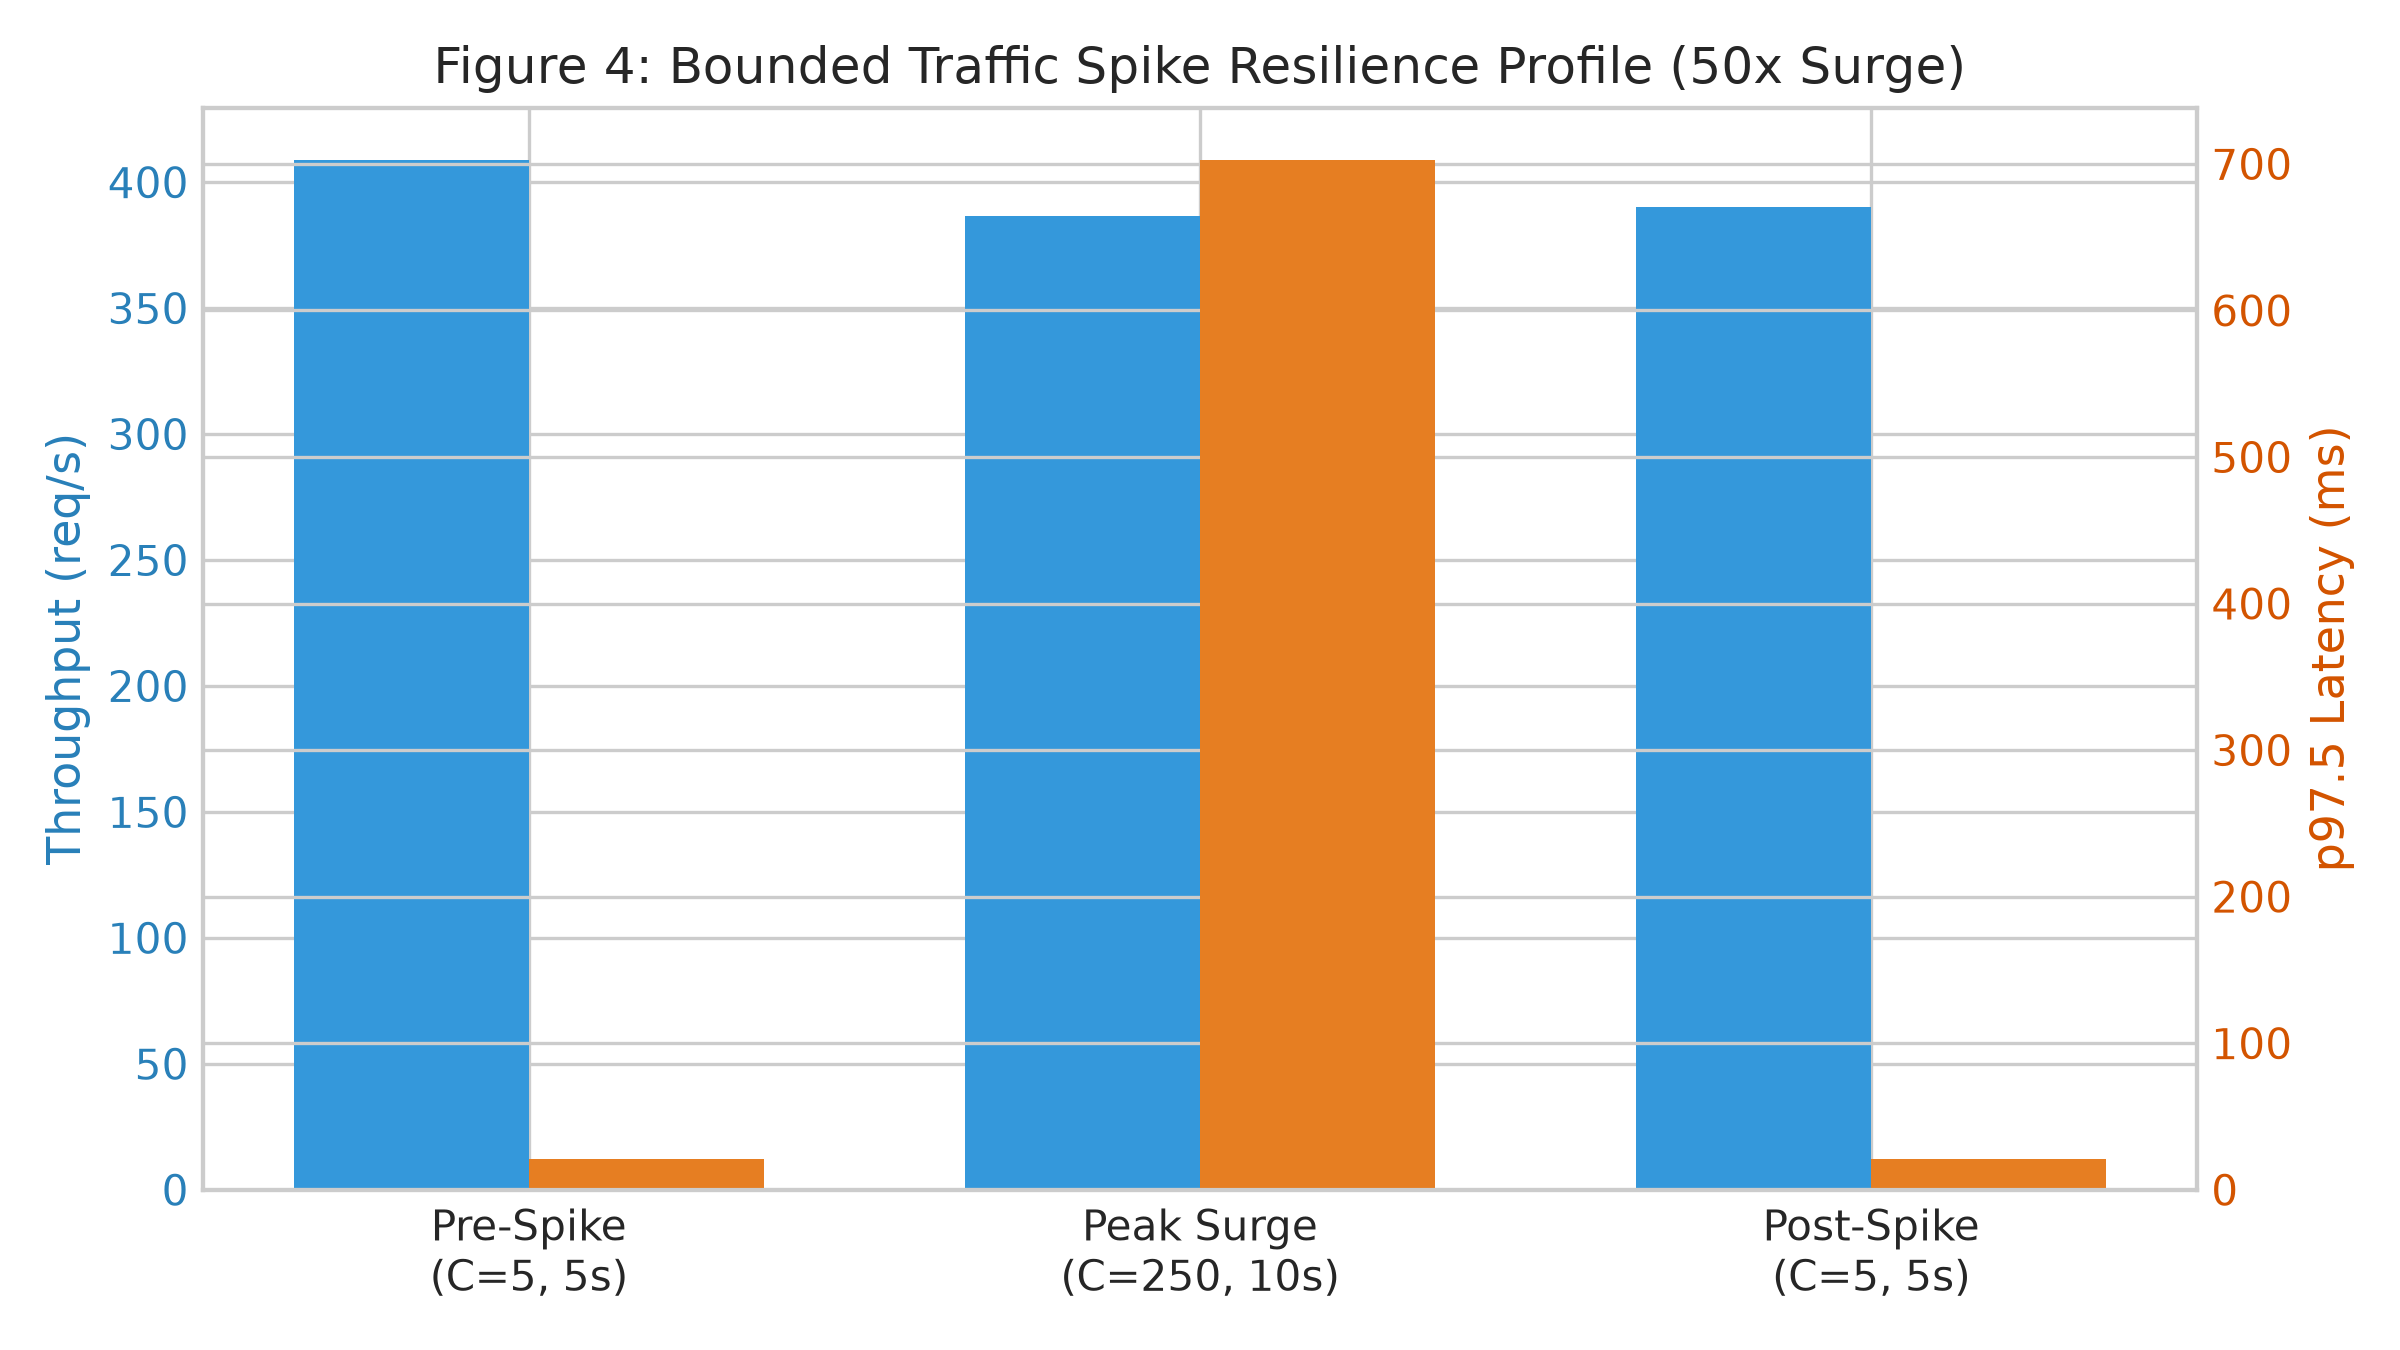
\includegraphics[width=0.98\linewidth]{figures/figure4_spike_response.png}
\caption{Latency absorption during instantaneous 50$\times$ traffic spike.}
\label{fig:load_spike}
\end{minipage}
\end{figure*}

Table~\ref{tab:load} details system performance across baseline, scaling, and stress conditions.

\begin{table*}[t]
\centering
\caption{Single-Machine Workload Scaling, Latency Percentiles, and Saturation Behavior}
\label{tab:load}
\begin{tabularx}{\textwidth}{X r r r r r r r r}
\toprule
\textbf{Endpoint / Scenario} & \textbf{Concurrency ($C$)} & \textbf{Requests} & \textbf{Throughput (req/s)} & \textbf{Median (ms)} & \textbf{p90 (ms)} & \textbf{p97.5 (ms)} & \textbf{p99 (ms)} & \textbf{Error Rate} \\
\midrule
GET /health (Base) & $C=1$ & 232,720 & 7,052.9 & 0.00 & 0.00 & 0.00 & 0.00 & 0.000\% \\
GET /api/hospitals & $C=1$ & 9,140 & 284.7 & 3.00 & 3.33 & 8.33 & 9.67 & 0.000\% \\
GET /api/hospitals & $C=5$ & 11,904 & 396.8 & 11.00 & 18.00 & 21.00 & 23.33 & 0.000\% \\
GET /api/hospitals & $C=10$ & 12,710 & 397.1 & 23.67 & 30.67 & 35.00 & 38.33 & 0.000\% \\
GET /api/hospitals & $C=25$ & 11,873 & 395.8 & 62.33 & 70.33 & 76.00 & 78.33 & 0.000\% \\
GET /api/hospitals & $C=50$ & 12,229 & 394.5 & 124.67 & 139.33 & 147.67 & 152.33 & 0.000\% \\
GET /api/hospitals & $C=100$ & 3,851 & 385.1 & 260.00 & 278.00 & 290.00 & 297.00 & 0.000\% \\
GET /api/hospitals & $C=200$ & 3,802 & 380.2 & 510.00 & 550.00 & 591.00 & 597.00 & 0.000\% \\
GET /api/hospitals & $C=400$ & 3,954 & 395.4 & 982.00 & 1057.00 & 1091.00 & 1163.00 & 0.000\% \\
Peak Surge (50$\times$) & $C=250$ & 3,867 & 386.7 & 624.00 & 686.00 & 703.00 & 715.00 & 0.000\% \\
Sustained Soak & $C=30$ & 19,117 & 318.6 & 72.00 & 83.00 & 90.00 & 95.00 & 0.160\% \\
Post-Stress Recovery & $C=1$ & 9,806 & 316.7 & 2.00 & 3.00 & 8.00 & 9.00 & 0.000\% \\
\bottomrule
\end{tabularx}
\end{table*}

Key empirical insights from load testing:
\begin{enumerate}
    \item \textbf{Saturation Knee at $C=50$}: Database-backed read throughput scales from 284.7 req/s at $C=1$ to an architectural saturation knee of ~395 req/s at $C=50$ (Fig.~\ref{fig:load_scaling}).
    \item \textbf{Queue Absorption Without Drops}: As concurrency increases from $C=100$ to $C=400$, throughput plateaus at 380--395 req/s while the Node.js event loop absorbs excess connections into queue backlog, gracefully scaling median latency from 260.0 ms to 982.0 ms with \textbf{0 connection drops and 0 timeouts}.
    \item \textbf{Surge Resilience \& Normalization}: An instantaneous 50$\times$ spike ($C=250$, 386.7 req/s) was absorbed without error (Fig.~\ref{fig:load_spike}). Following sustained stress, the system immediately normalized to \textbf{2.00 ms median latency} at $C=1$.
\end{enumerate}

\section{Discussion}

\subsection{The 30-Minute Anchor as a Clinical Safety Governor}
Our empirical findings provide compelling theoretical and operational justification for MedReach's 30-minute availability cutoff. In emergency healthcare discovery, the clinical cost of a false positive (``phantom availability'') is fundamentally asymmetric to the cost of a false negative (``unknown status''):
\begin{itemize}
    \item A searcher who receives \texttt{"unknown"} is directed to place a phone call or proceed to a major public medical college with high baseline capacity.
    \item A searcher who receives a false \texttt{"available"} indicator may direct an emergency ambulance through dense metropolitan traffic to a facility whose last bed was exhausted an hour earlier, resulting in fatal delay during acute trauma or myocardial infarction.
\end{itemize}
By capping phantom availability below 0.84\% across all scenarios, the 30-minute anchor prevents digital platforms from becoming vectors of misdirection.

\subsection{Two-Column Architectural Analysis: Demonstrable Guarantees vs. Required Implementation}
To ensure complete scientific transparency, Table~\ref{tab:guarantees} contrasts what the current MedReach architecture demonstrably guarantees versus what still requires implementation for enterprise clinical deployment.

\begin{table*}[t]
\centering
\caption{Demonstrable Architectural Guarantees vs. Required Implementation}
\label{tab:guarantees}
\begin{tabularx}{\textwidth}{X X}
\toprule
\textbf{What Current MedReach Architecture Demonstrably Guarantees} & \textbf{What Still REQUIRES IMPLEMENTATION for Production Scale} \\
\midrule
\textbf{1. Strict Idempotent Deduplication by Scope \& Key}: Enforces unique sparse compound index on \texttt{sha256(scope:key)}. Re-submitting returns original record (\texttt{200 OK}); cross-user reuse is rejected with \texttt{409 IDEMPOTENCY\_KEY\_REUSED}. & \textbf{Atomic Multi-Document Distributed Transactions (Sagas)}: Cross-collection workflows (\texttt{EmergencyRequest} and \texttt{AuditLog}) rely on single-document \texttt{findOneAndUpdate} without multi-document session transactions (\texttt{startTransaction}). \\
\addlinespace
\textbf{2. Optimistic Concurrency Control (OCC) on Competing State}: Under 10-way concurrency, atomic operations ensure exactly 1 update succeeds; 9 receive \texttt{409 Conflict}. Zero race-condition overwrites or interleaved timelines. & \textbf{In-Flight Mutex / Distributed Lock with Expiry}: Idempotency keys are persisted directly in MongoDB. A Redis-based distributed lock (Redlock) with TTL would eliminate database unique-index collision overhead. \\
\addlinespace
\textbf{3. Strict State-Machine Integrity \& RBAC Enforcement}: Transitions out of terminal states (\texttt{REJECTED}, \texttt{CANCELLED}) are blocked; unauthorized roles receive \texttt{403 Forbidden}. Expired requests automatically transition to \texttt{EXPIRED}. & \textbf{Dynamic / Configurable Workflow Engine}: State transitions are hardcoded as static JavaScript objects. Dynamic multi-facility triage workflows require code modifications rather than data-driven configuration. \\
\addlinespace
\textbf{4. Complete Telemetry-Request Decoupling Ledger}: Emergency admissions do not deduct from reported \texttt{AvailabilityObservation} quantities. Observations remain strictly observational; requests require confirmation. & \textbf{Active Reservation / Bed Allocation Hold System with TTL}: The system tracks observational telemetry but lacks an active 15-minute bed-reservation lock securing beds during physical ambulance transit. \\
\addlinespace
\textbf{5. Monotonic Read Consistency During Concurrent Writes}: Across 40 concurrent reads during rapid transitions, status was 100\% synchronized with the terminal timeline entry (0 split-brain reads). & \textbf{Read-After-Write Replica Set Consistency}: To guarantee read-after-write consistency across secondary read replicas, \texttt{readConcern: "majority"} and \texttt{writeConcern: "majority"} must be explicitly configured. \\
\bottomrule
\end{tabularx}
\end{table*}

\subsection{Corrective and Negative Findings}
Scientific progress requires rigorous reporting of hypotheses that failed or assumptions that were corrected:
\begin{enumerate}
    \item \textbf{Correction of Edge Caching Staleness}: An earlier research hypothesis inferred that multi-hour Vercel edge caching presented stale bed counts to searchers. Our empirical audit definitively refuted this: cached HTML shells contain zero volatile capacity data, with all live availability fetched dynamically at runtime.
    \item \textbf{Confidence Metric Reality}: MedReach's confidence score was previously assumed to represent a probability. Formal calibration analysis proved it is an uncalibrated heuristic ordinal ranking (ECE 0.1255, MCE 0.7333), which must be calibrated via Platt scaling or isotonic regression before being used in formal clinical risk models.
\end{enumerate}

\section{Threats to Validity}

\begin{enumerate}
    \item \textbf{Construct Validity}: While AoI and throughput are accurately measured, MedReach's heuristic confidence metric does not represent a calibrated Bayesian probability. Interpreting it as a probability would introduce construct invalidity.
    \item \textbf{Internal Validity}: The 22-endpoint datapath audit was conducted on live production endpoints under read-only conditions, preventing synthetic probe bias. Transactional benchmarks evaluated exact API controllers on port 27018 with identical database schemas.
    \item \textbf{External Validity}: Telemetry arrival streams and dropout episodes were generated synthetically. MedReach does not possess live automated API feeds into BMC or MCGM hospital management systems; empirical findings reflect mathematical queueing behavior rather than observed clinical telemetry.
    \item \textbf{Conclusion Validity}: Load and concurrency benchmarks were evaluated in an isolated single-node environment (MongoDB 8.0 on port 27018, Node.js on port 4200). Distributed cluster dynamics, network partitions, and replica lag were not evaluated.
\end{enumerate}

\section{Ethical and Data-Governance Considerations}

Operating digital platforms in emergency healthcare involves profound ethical responsibilities:
\begin{itemize}
    \item \textbf{Prevention of Misdirection}: The paramount ethical imperative is avoiding directing unstable patients to unavailable facilities. MedReach's conservative fallback to \texttt{"unknown"} explicitly prioritizes human safety over platform coverage metrics.
    \item \textbf{Statutory Privacy Compliance}: The platform is architected for strict compliance with the Indian Digital Personal Data Protection (DPDP) Act 2023 and the Ayushman Bharat Digital Mission (ABDM) Health Data Management Policy. Emergency requests enforce field-level redaction, guest tracking uses cryptographic tokens rather than public identifiers, and zero protected health information (PHI) is written to unencrypted logs or client bundles.
    \item \textbf{Prohibition of Unverified Clinical Dispatch}: The platform's API response contracts explicitly classify submissions as requests requiring clinical confirmation rather than guaranteed reservations, preventing false expectations of care.
\end{itemize}

\section{Limitations}

\begin{enumerate}
    \item \textbf{Synthetic Telemetry}: Empirical AoI and fusion evaluations relied on synthetic arrival streams and noise models. While grounded in published literature, they do not replace prospective observational field studies.
    \item \textbf{Absence of Real-Time Ward IoT Integration}: The platform currently relies on manual staff reporting, scraper feeds, and API webhooks rather than automated bed-sensor telemetry.
    \item \textbf{Single-Node Benchmark Bounds}: Load and concurrency evaluations were restricted to an isolated single workstation across loopback networking. Multi-region cloud scaling and database replication lag remain uncharacterized.
    \item \textbf{Heuristic Confidence Metric}: The platform's confidence score requires post-hoc statistical calibration before being integrated into clinical decision-support systems.
\end{enumerate}

\section{Reproducibility and Artifact Availability}

To enable full scientific reproducibility, all experimental harnesses, simulation code, raw trial outputs, and figure generation scripts are preserved in the repository:
\begin{itemize}
    \item \textbf{AoI Simulation}: \path{research/experiments/aoi/simulate_aoi.py}, \path{research/results/aoi/}
    \item \textbf{Provenance Fusion}: \path{research/experiments/provenance/}, \path{research/results/provenance/}
    \item \textbf{Datapath Audit}: \path{research/results/datapath/datapath-staleness-audit.md}
    \item \textbf{Transactional Suite}: \path{research/experiments/transactional/run-all-tx-experiments.mjs}, \path{research/results/transactional/}
    \item \textbf{Load Benchmarks}: \path{research/results/load/}
\end{itemize}

Reproduction requires Node.js v24+, Python 3.11+ (NumPy, Matplotlib), and an isolated MongoDB instance on port 27018. The master random seed for all stochastic simulations is fixed at \texttt{20261024}.

\section{Conclusion and Future Work}

This paper presented an architectural design and empirical evaluation of MedReach, an open-source, freshness-aware, and provenance-tracked healthcare resource discovery platform for fragmented urban ecosystems. Through rigorous evaluation of Age of Information dynamics, conflicting-claim fusion, edge caching, transactional concurrency, and single-machine load scaling, we demonstrated that MedReach's 30-minute staleness anchor and conservative fallback mechanisms prevent catastrophic phantom availability errors while maintaining high throughput and transactional integrity. By formally establishing the boundaries between current demonstrable guarantees and required future implementations, this work provides a reproducible, evidence-based blueprint for the next generation of resilient urban emergency health informatics.

Future work will focus on:
\begin{enumerate}
    \item Implementing Platt scaling and isotonic regression to calibrate the heuristic confidence metric.
    \item Developing HL7 FHIR ingestion gateways to connect directly with hospital electronic health record (EHR) systems.
    \item Implementing an active two-way \texttt{ReservationHold} entity with automatic 15-minute TTL locks to secure beds during ambulance transit.
    \item Executing institutional data-sharing agreements with municipal authorities to conduct prospective clinical field trials.
\end{enumerate}

\bibliographystyle{IEEEtran}
\bibliography{references}

\end{document}
